\section{Diagrammi di attività}

Vengono in seguito illustrati i diagrammi di attività prodotti durante la progettazione architetturale, i quali descrivono le iterazioni dell'utente con il sistema \glossario{MaaP}. È stato scelto di dividere i diagrammi in due categorie principali, in modo analogo a quanto fatto nella descrizione dei casi d'uso dell'\textit{Analisi dei requisiti}:

\begin{itemize}

	\item \textbf{Applicazione \glossario{MaaP}}, in cui verranno descritte le iterazioni che un utente può fare all'interno di un'applicazione generata dal \glossario{framework};
	\item \textbf{Framework \glossario{MaaP}}, in cui verrà descritto il modo in cui uno sviluppatore può creare un'applicazione.

\end{itemize}

Inizialmente per ogni categoria verrà fornito uno schema ad alto livello, per poi andare sempre più nel dettaglio tramite sotto-diagrammi più specifici. Per comodità di visualizzazione le attività che verranno \textit{esplose} sono marcate in grassetto. 

Al fine di rendere il diagramma leggibile abbiamo considerato implicito il fatto che un utente possa in qualsiasi momento uscire dall'applicazione \glossario{MaaP}, per esempio chiudendo la finestra del browser.

\subsection{Applicazione MaaP}

Vengono di seguito descritte tutte le iterazioni che un utente può effettuare con un'applicazione generata dal \glossario{framework} \glossario{MaaP}.


\subsubsection{attività principali}

\begin{figure}[H]
\centering
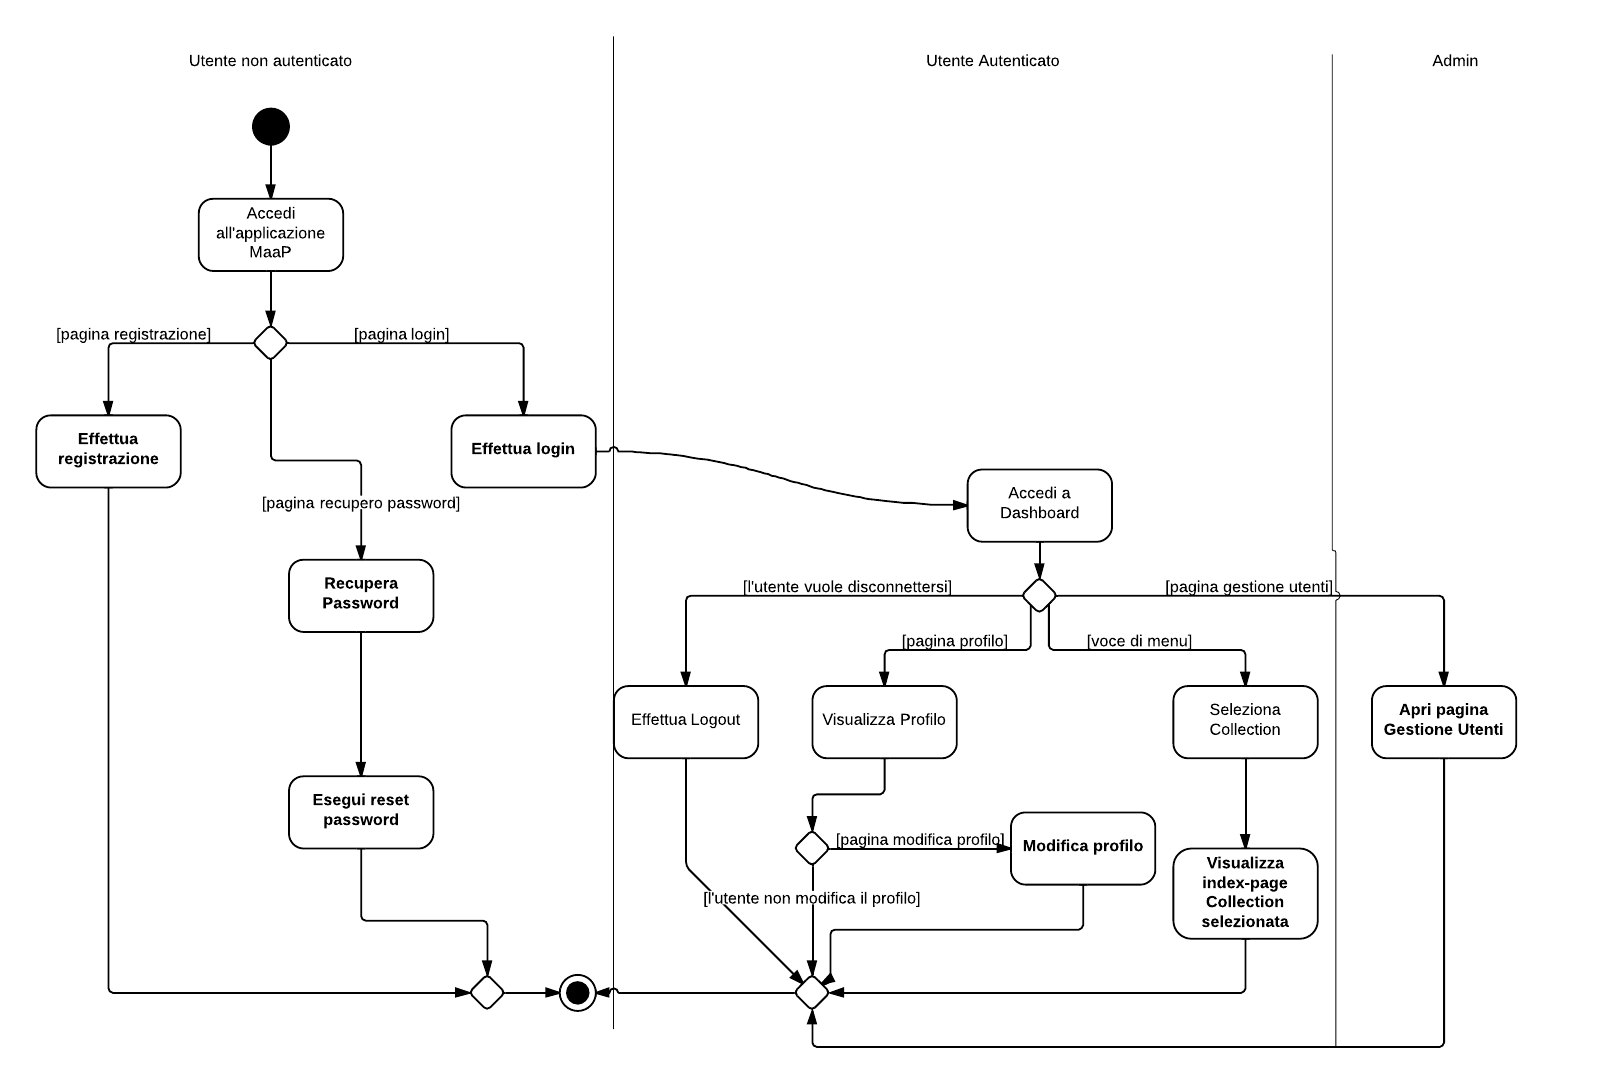
\includegraphics[scale=0.3]{uml/attivita/MaaP - Attivita principali.png}
\caption{Diagramma di attività - attività principali di un'applicazione MaaP}
\end{figure}

Sostanzialmente un'applicazione generata da \glossario{MaaP} è composta da una serie di pagine web all'interno delle quali un utente può navigare. Un utente accede inizialmente all'applicazione web in una pagina statica in cui può effettuare tre cose:

\begin{itemize}

	\item Registrarsi al sistema;
	\item Effettuare il login;
	\item Recuperare la propria password.

\end{itemize}

Una volta che l'utente ha effettuato il login viene direttamente indirizzato alla \glossario{Dashboard}, dalla quale può navigare all'interno dell'applicazione ed effettuare diverse operazioni:

\begin{itemize}

	\item Effettuare il logout;
	\item Visualizzare il proprio profilo e di conseguenza modificarlo;
	\item Selezionare una \glossario{Collection} esistente.

\end{itemize}

Nel caso in cui l'utente avesse i privilegi di admin può inoltre accedere ad una specifica pagina di gestione degli utenti iscritti.

\subsubsection{Effettua registrazione}

\begin{figure}[H]
\centering
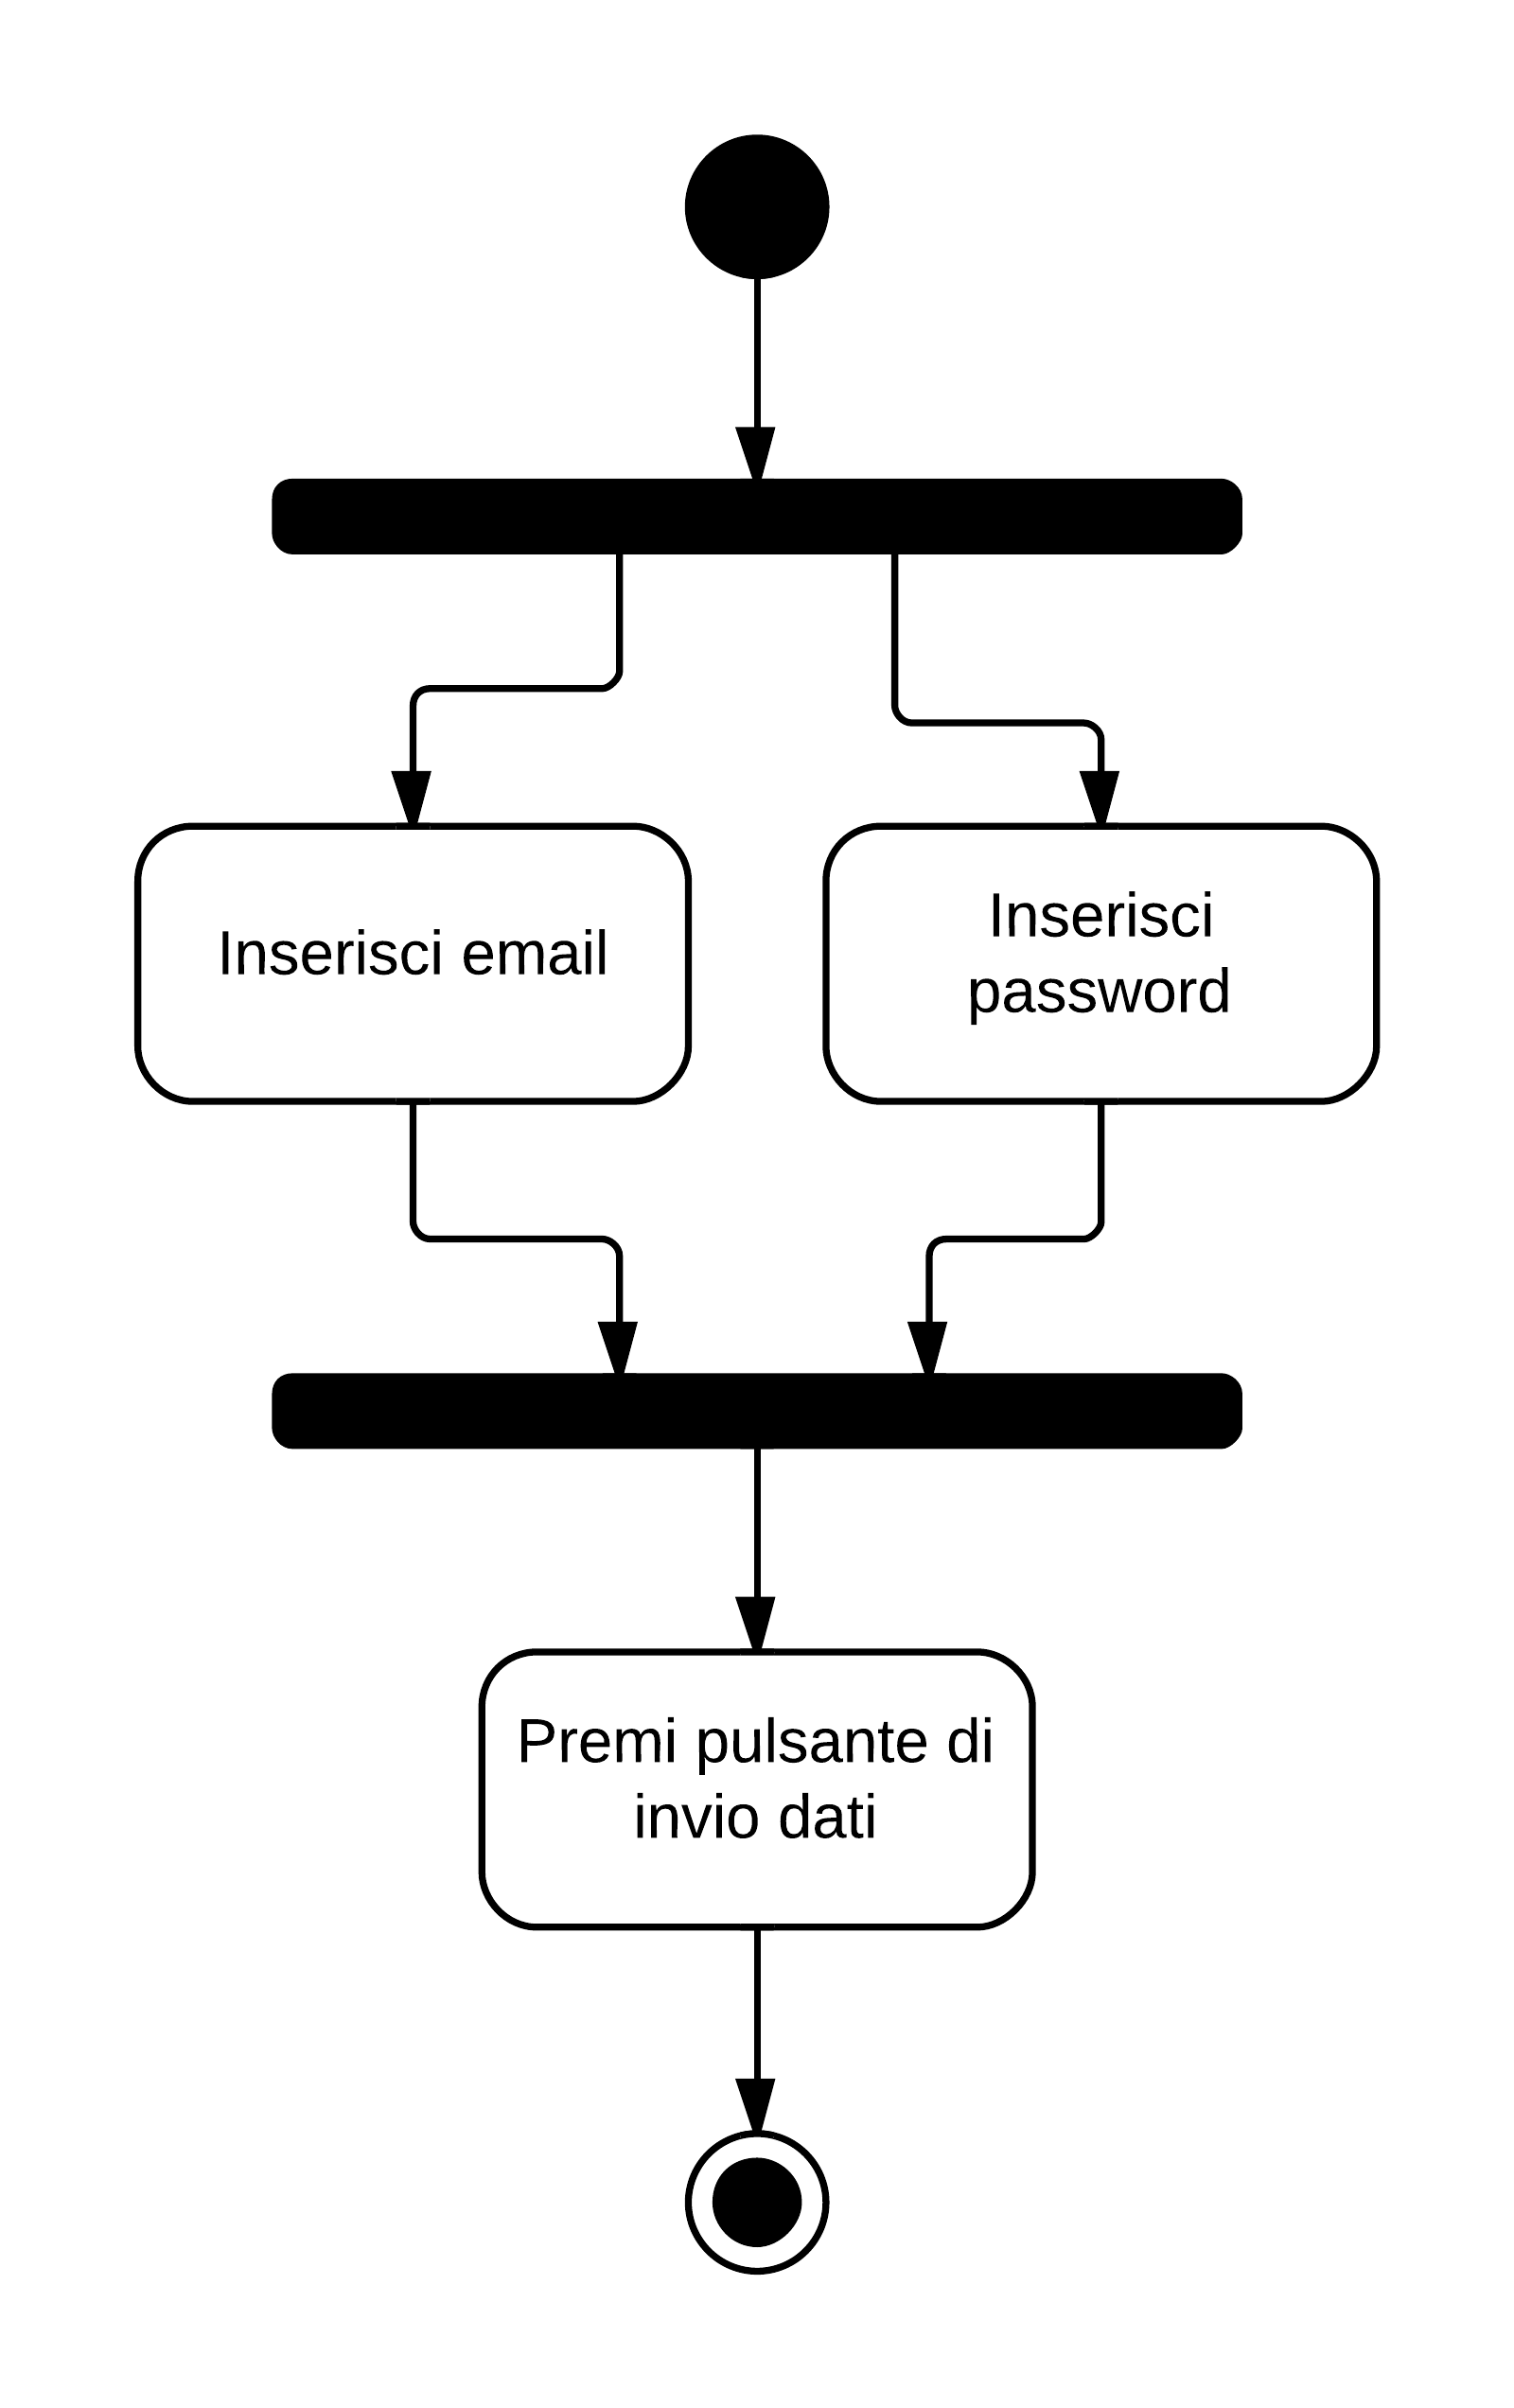
\includegraphics[scale=0.1]{uml/attivita/MaaP - Effettua registrazione.png}
\caption{Diagramma di attività - Registrazione di un utente}
\end{figure}

L'utente si trova all'interno della pagina di registrazione e sostanzialmente deve inserire la propria email e la propria password all'interno di due campi di testo. Una volta inseriti l'utente deve premere il pulsante di invio dati; il sistema \glossario{MaaP} procederà dunque alla verifica delle credenziali e, se quest'ultima avrà successo, alla registrazione dell'utente.

\subsubsection{Recupera password}

\begin{figure}[H]
\centering
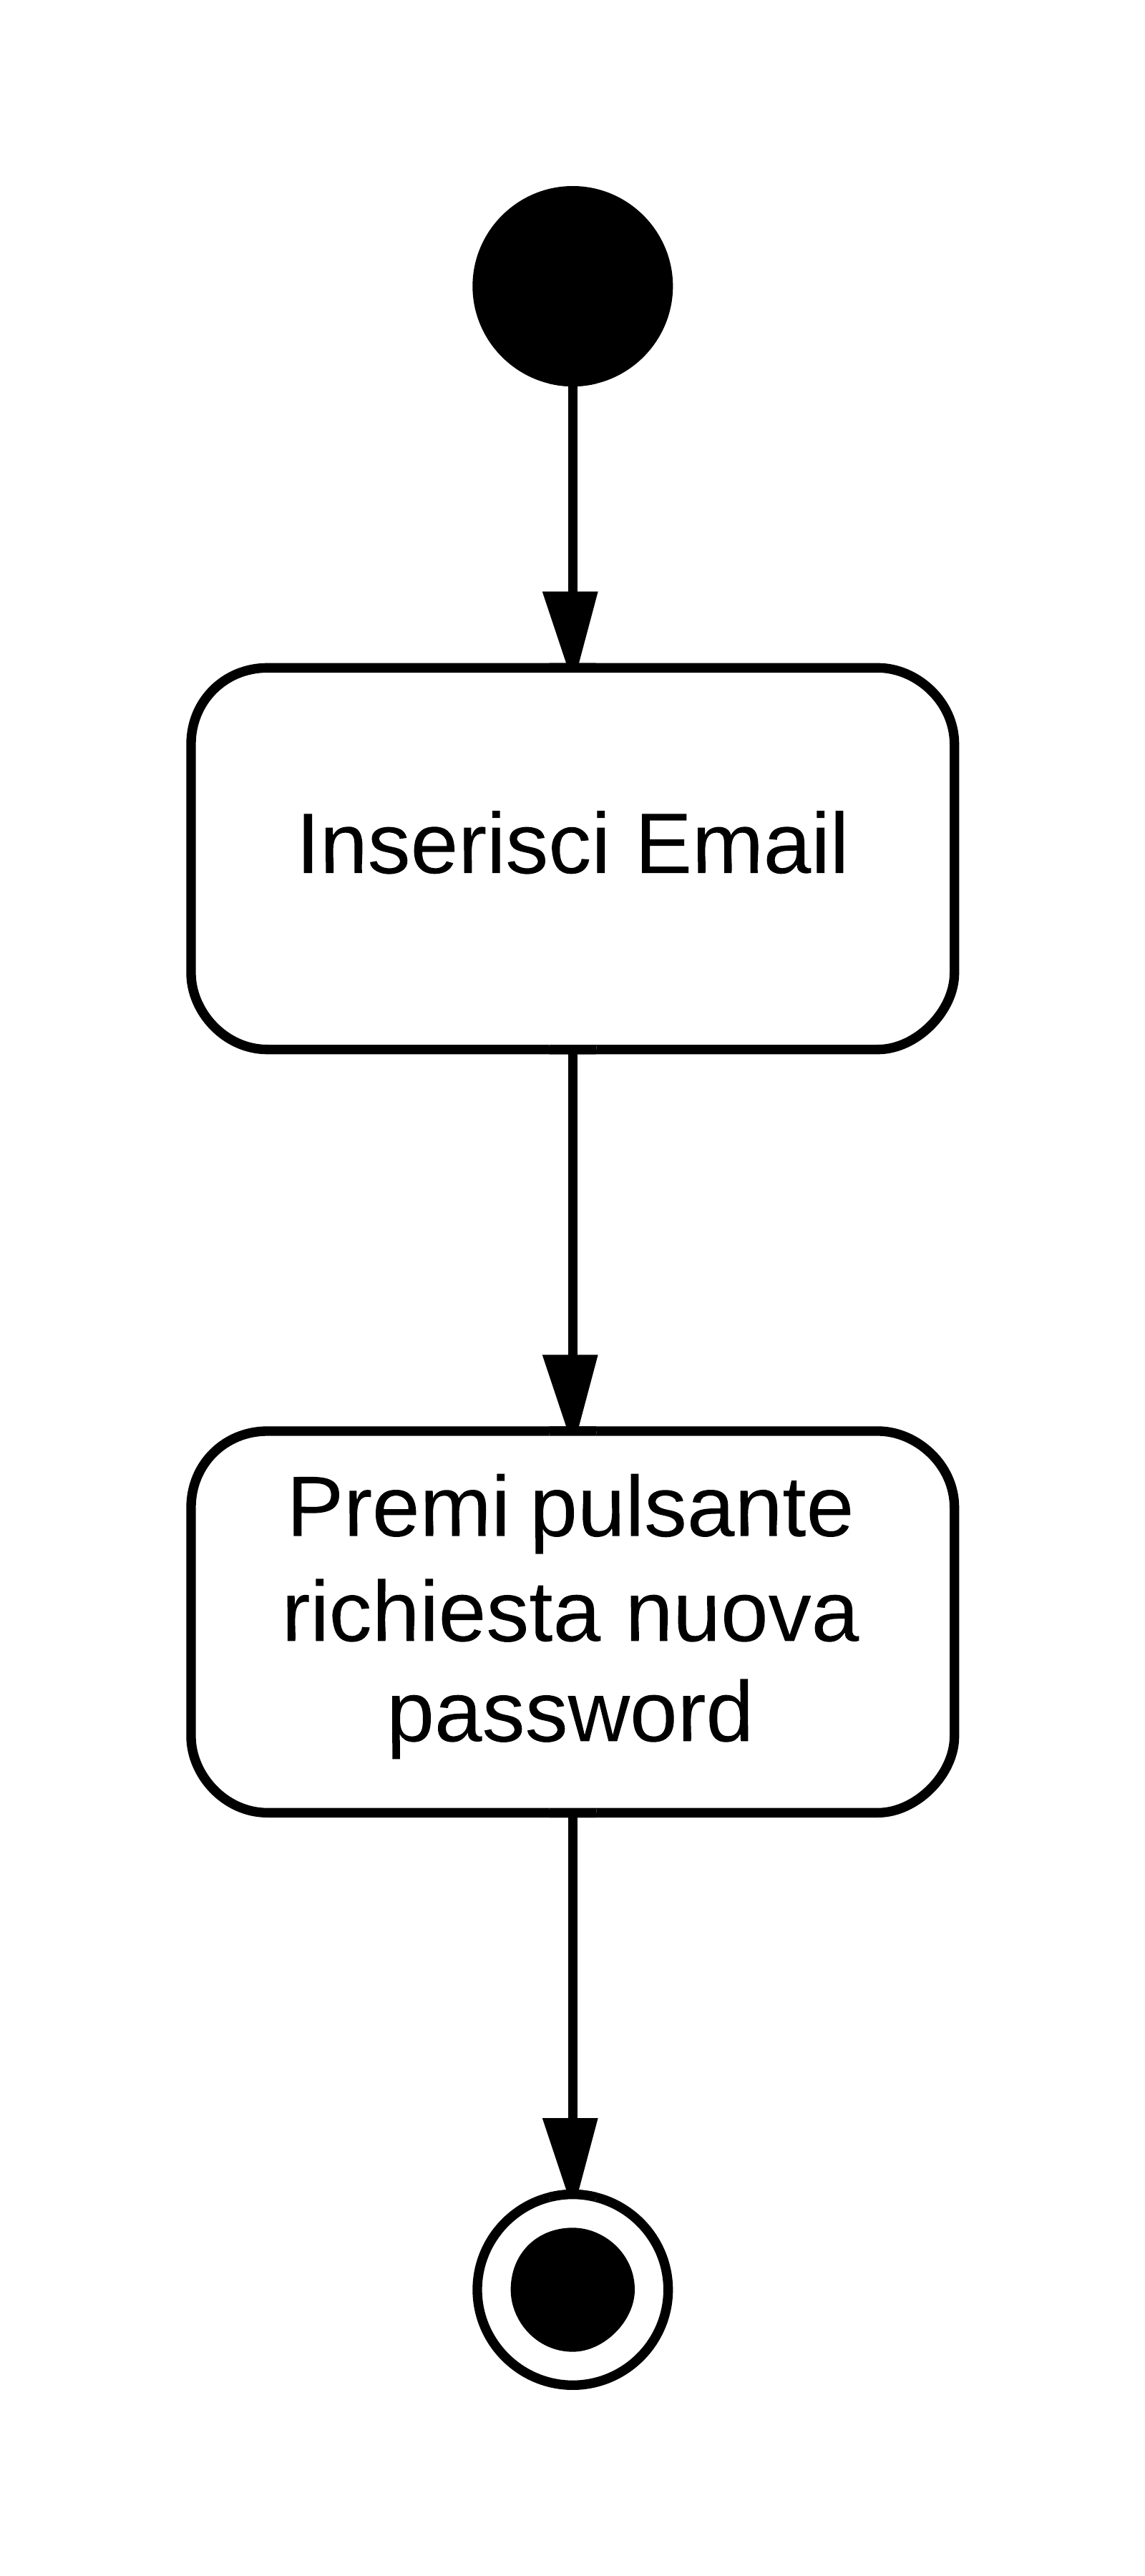
\includegraphics[scale=0.05]{uml/attivita/MaaP - Recupera password.png}
\caption{Diagramma di attività - Recupero password}
\end{figure}

L'utente si trova all'interno della pagina di recupero password, la quale presenta un campo di testo nel quale l'utente dovrà inserire il proprio indirizzo email. Una volta inserito preme il pulsante di richiesta di una nuova password; il sistema \glossario{MaaP} procederà dunque alla verifica dell'indirizzo email e, se quest'ultima avrà esito positivo, invierà un'email all'utente con le relative istruzioni per il ripristino della password.

\subsubsection{Esegui reset password}

\begin{figure}[H]
\centering
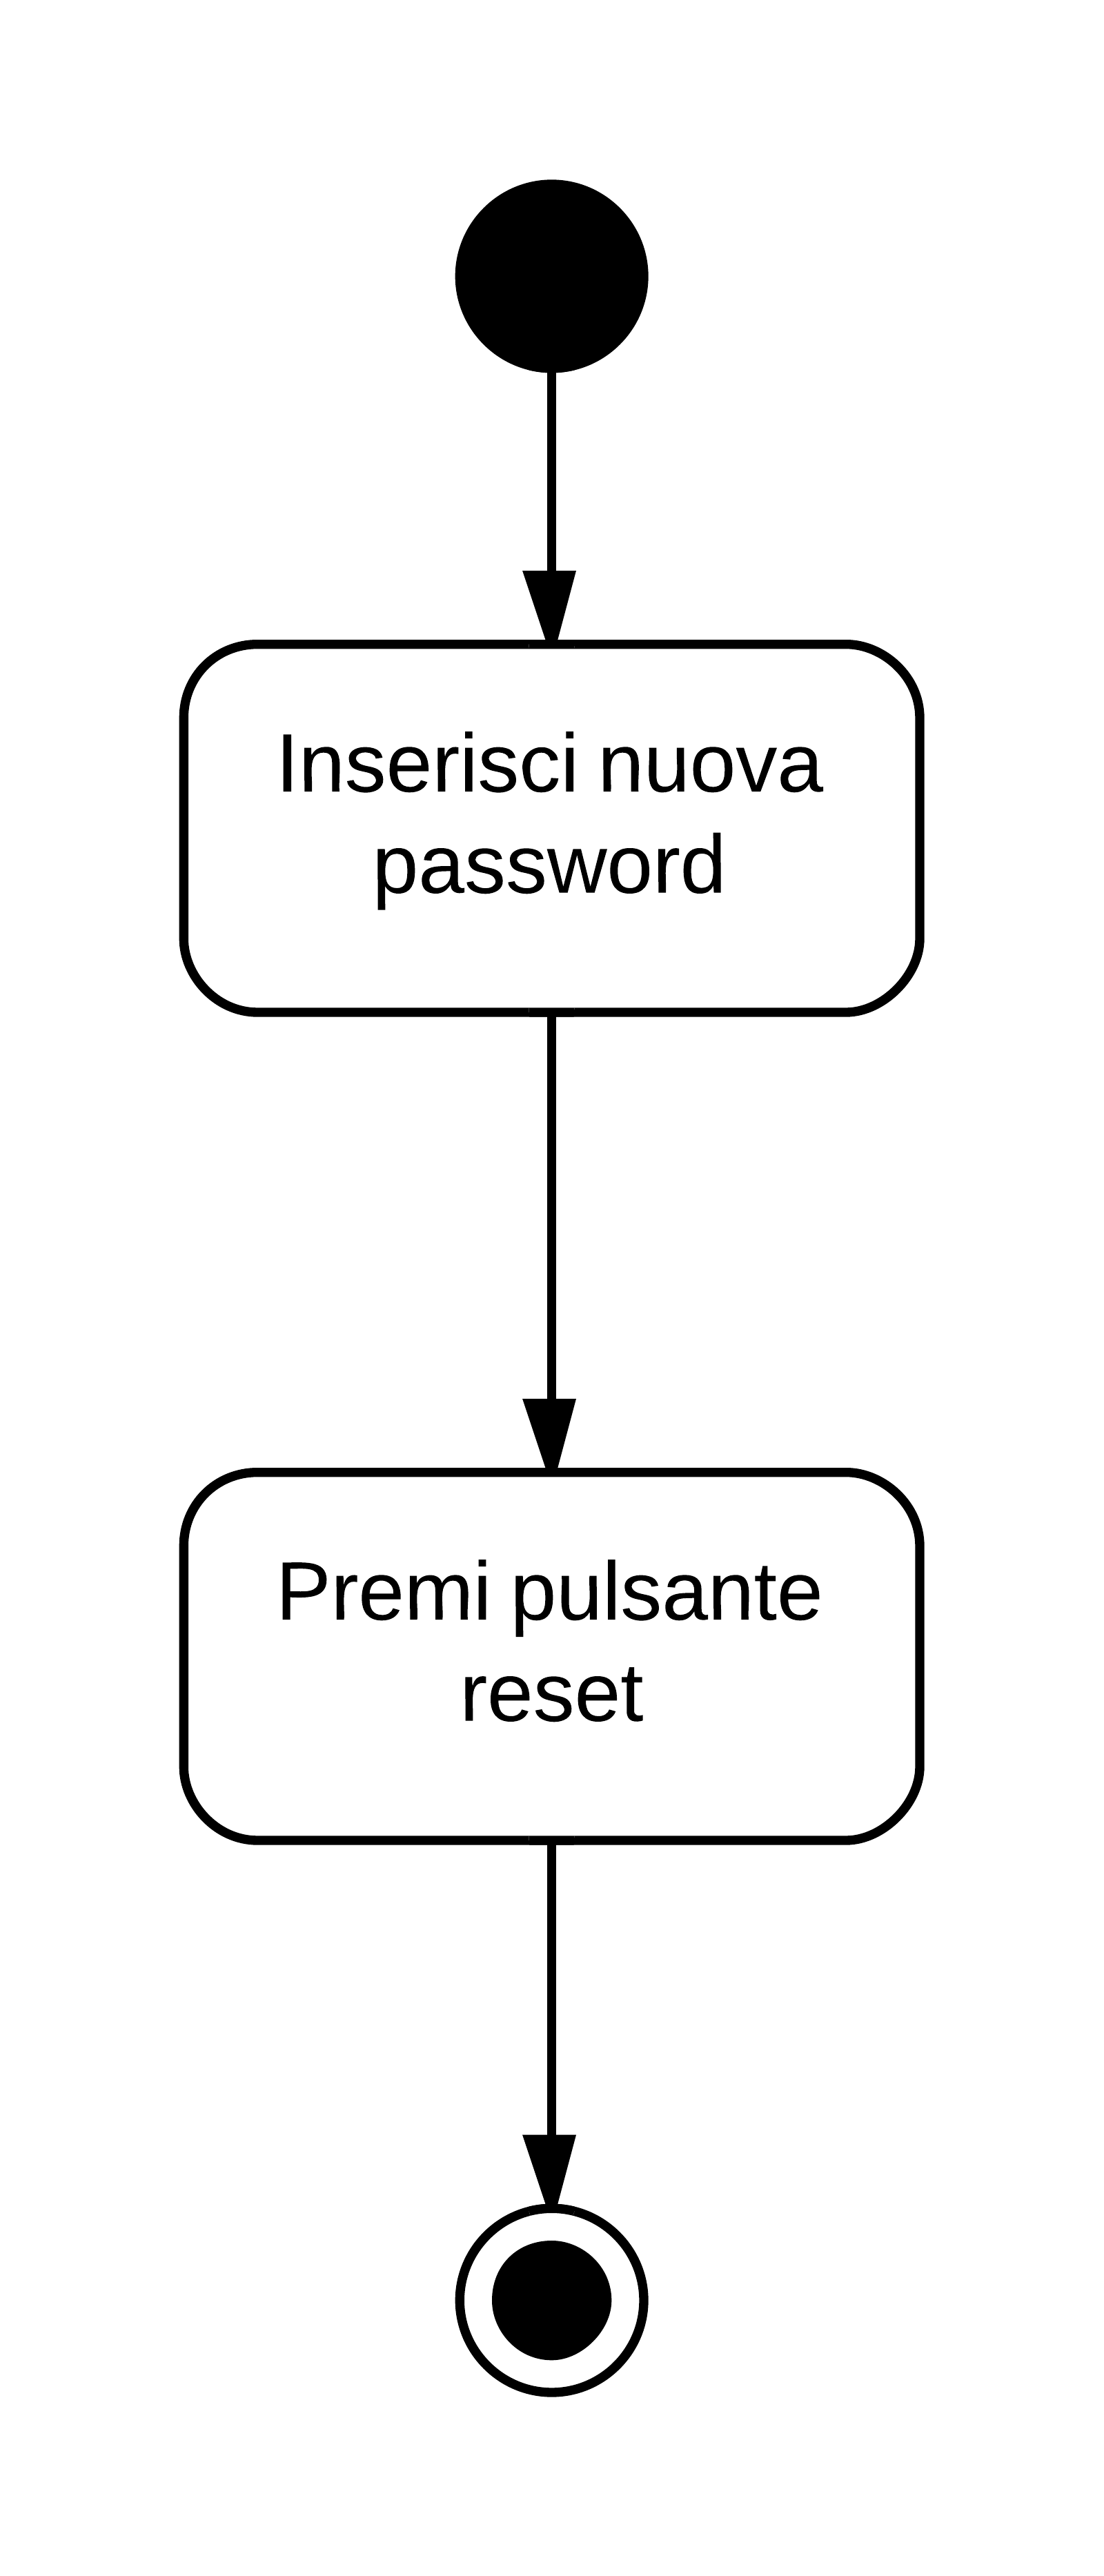
\includegraphics[scale=0.05]{uml/attivita/MaaP - Esegui reset password.png}
\caption{Diagramma di attività - Reset della password dell'utente}
\end{figure}

L'utente avrà ricevuto un'email con al suo interno un link ad una pagina univoca dell'applicazione \glossario{MaaP} e quindi si troverà in una pagina con al suo interno un campo di testo nel quale inserire la nuova password. Una volta inserita la password deve premere il pulsante di reset; il sistema \glossario{MaaP} procederà dunque al cambio password per l'utente corrente nel \glossario{database} delle credenziali.

\subsubsection{Effettua login}

\begin{figure}[H]
\centering
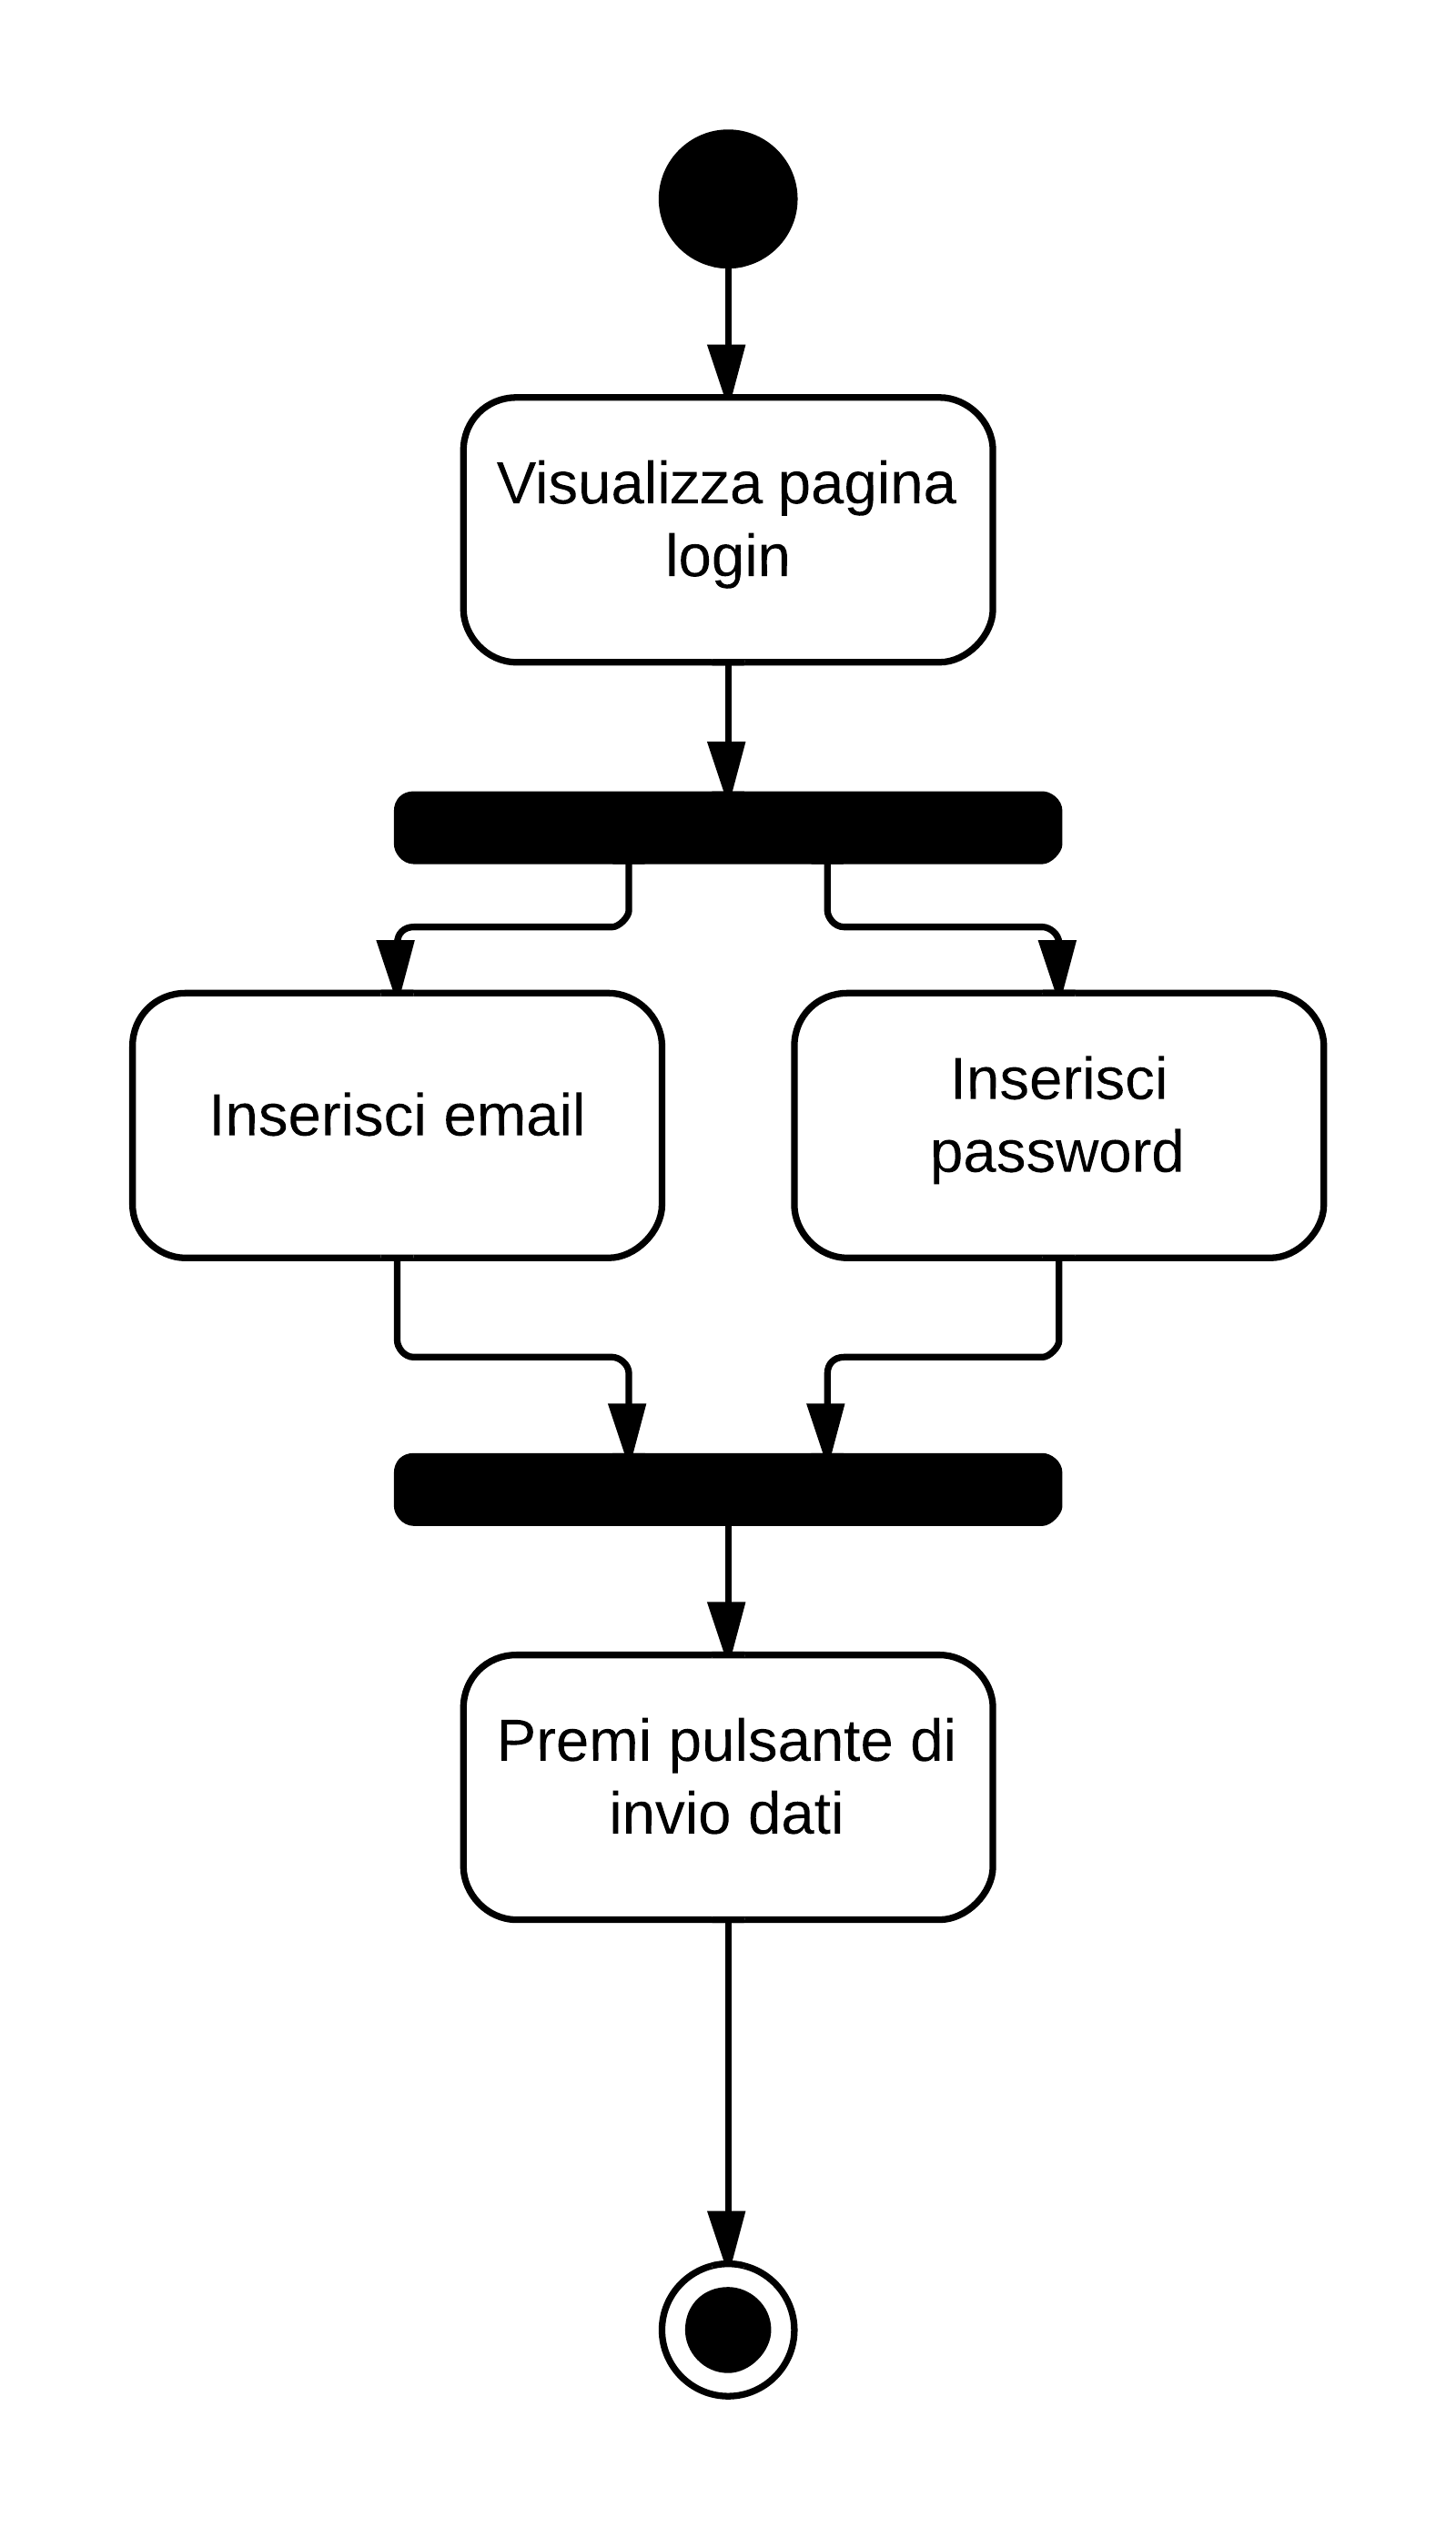
\includegraphics[scale=0.1]{uml/attivita/MaaP - Effettua login.png}
\caption{Diagramma di attività - Login dell'utente}
\end{figure}

L'utente, che precedentemente avrà effettuato la registrazione al sistema, accede all'interno dell'applicazione tramite una pagina di login. Al suo interno saranno presenti due campi di testo in cui l'utente dovrà inserire la propria email e la propria password. Una volta inserite dovrà premere il pulsante di login; il sistema \glossario{MaaP} procederà dunque alla verifica delle credenziali e, se l'esito di tale verifica risulterà positivo, effettuerà il login dell'utente all'applicazione, reindirizzandolo alla \glossario{dashboard}.

\subsubsection{Modifica profilo}

\begin{figure}[H]
\centering
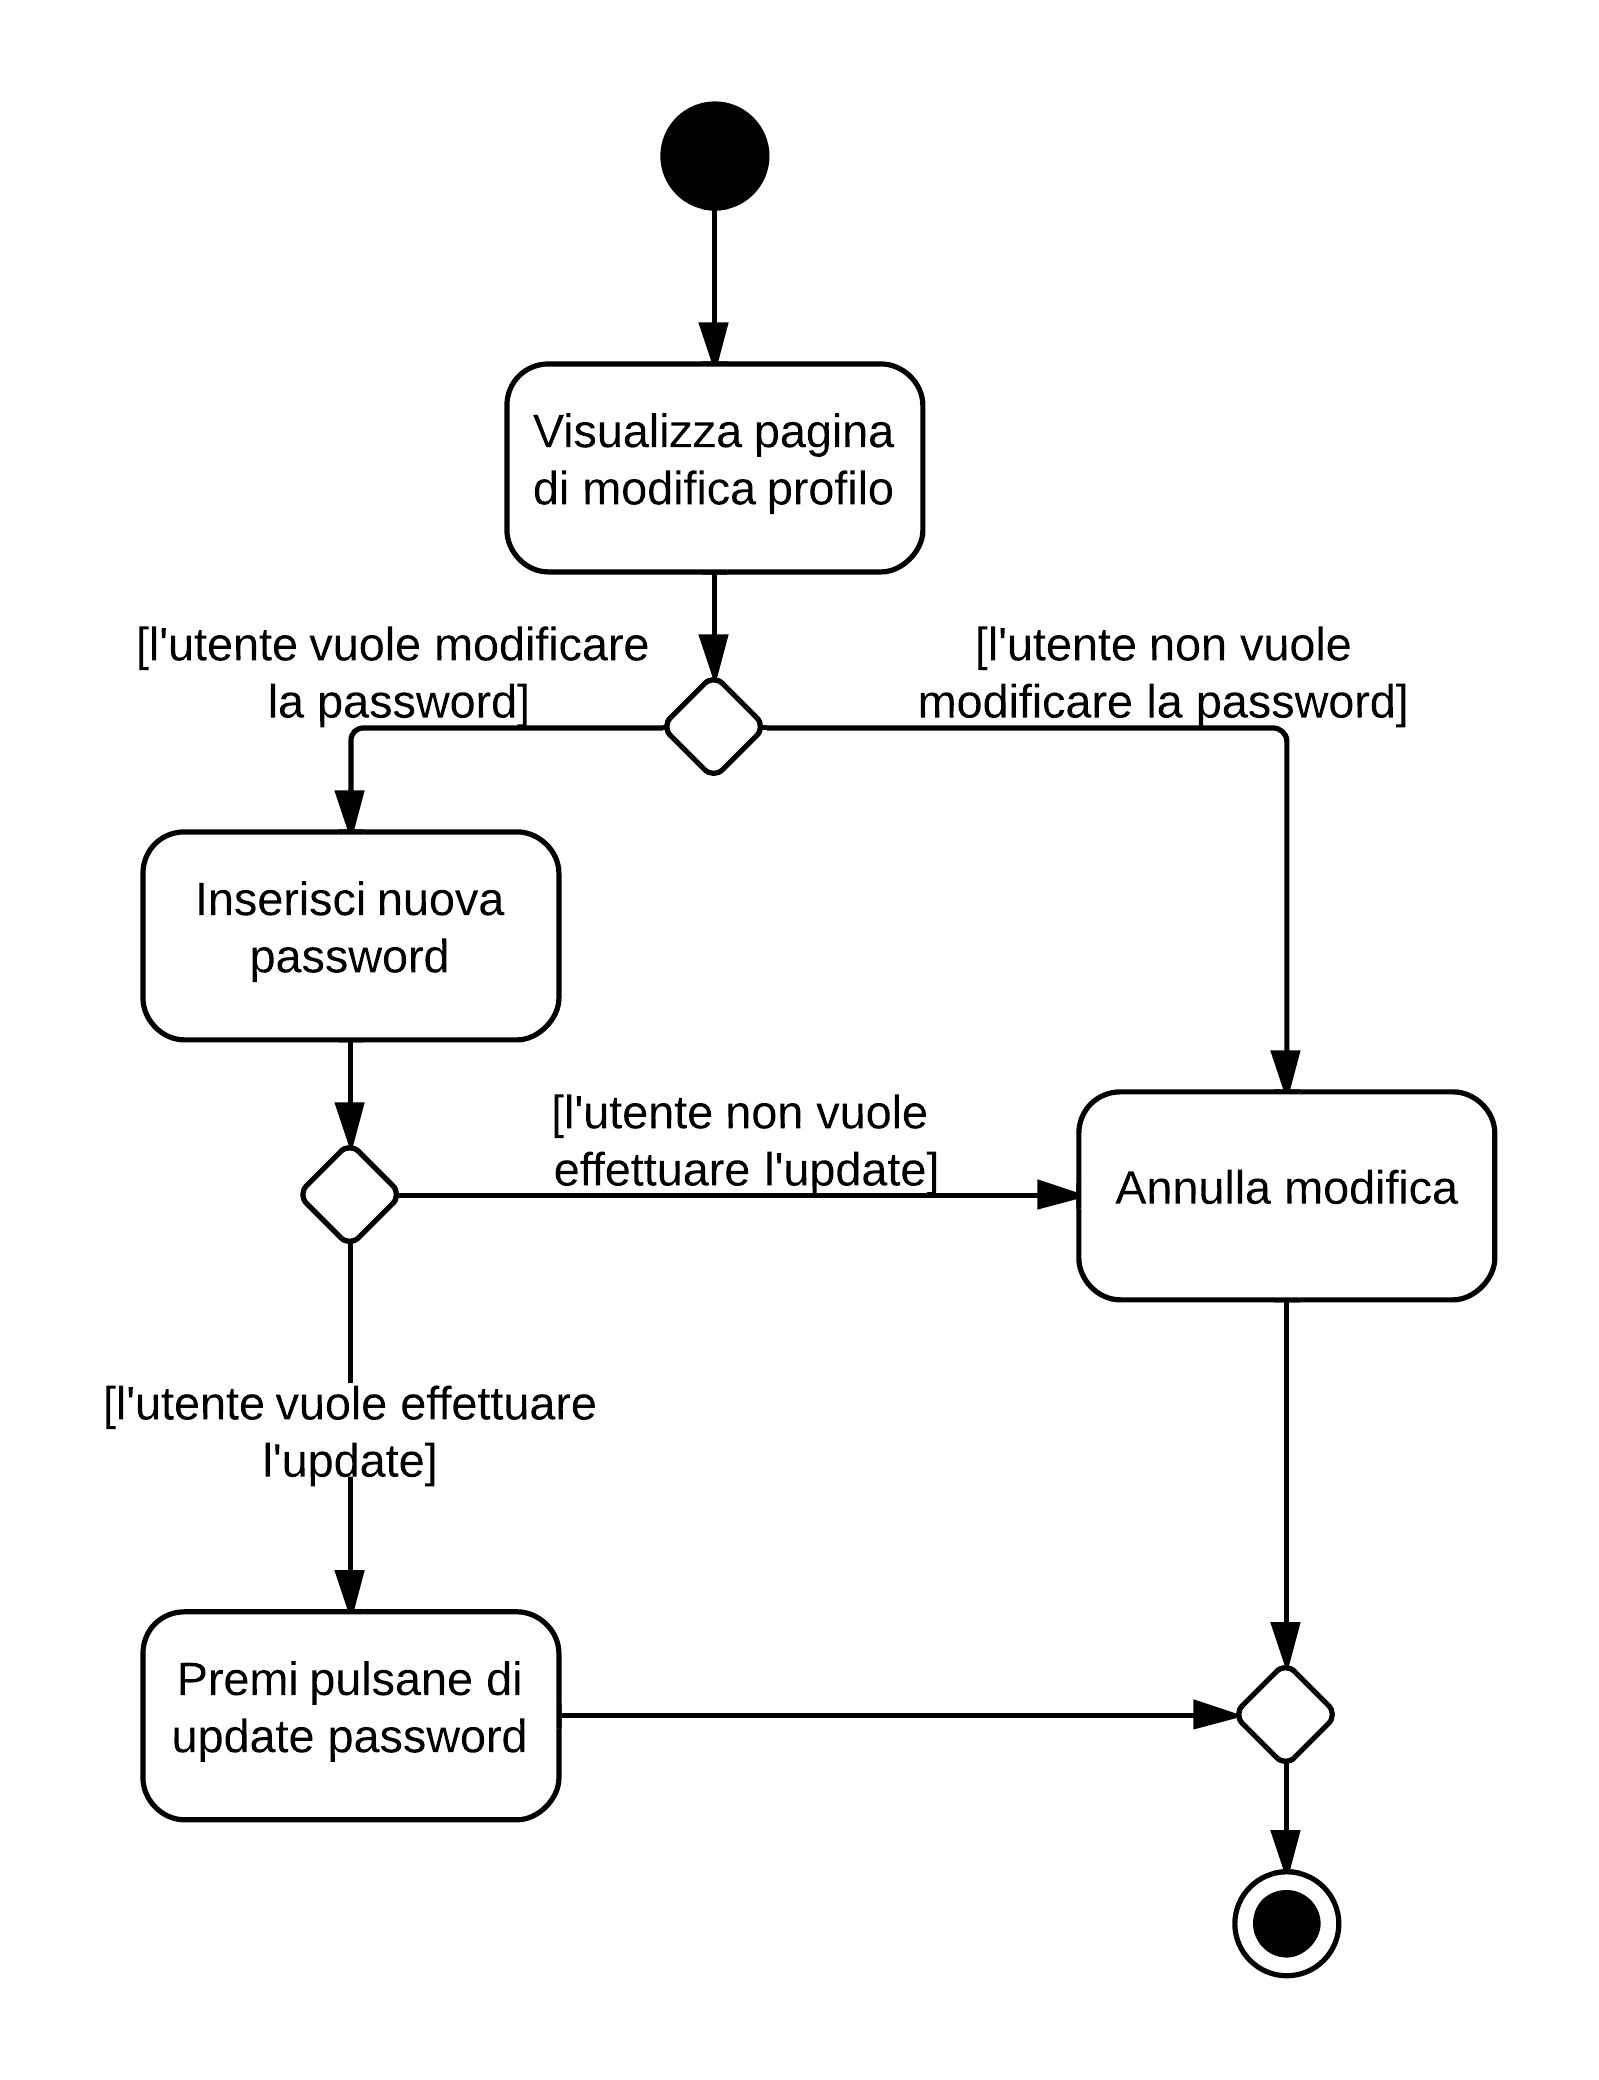
\includegraphics[scale=0.1]{uml/attivita/MaaP - Modifica profilo.png}
\caption{Diagramma di attività - Modifica profilo utente}
\end{figure}

L'utente autenticato accede all'interno della propria pagina profilo, dalla quale può decidere di modificare la propria password. Sarà dunque presente un campo di testo in cui l'utente inserirà la nuova password e un bottone tramite il quale invierà la richiesta di modifica; il sistema \glossario{MaaP} procederà dunque alla modifica della password dell'utente. L'utente in ogni momento può decidere di annullare le modifiche e tornare alla pagina precedente.

\subsubsection{Index-page Collection}

\begin{figure}[H]
\centering
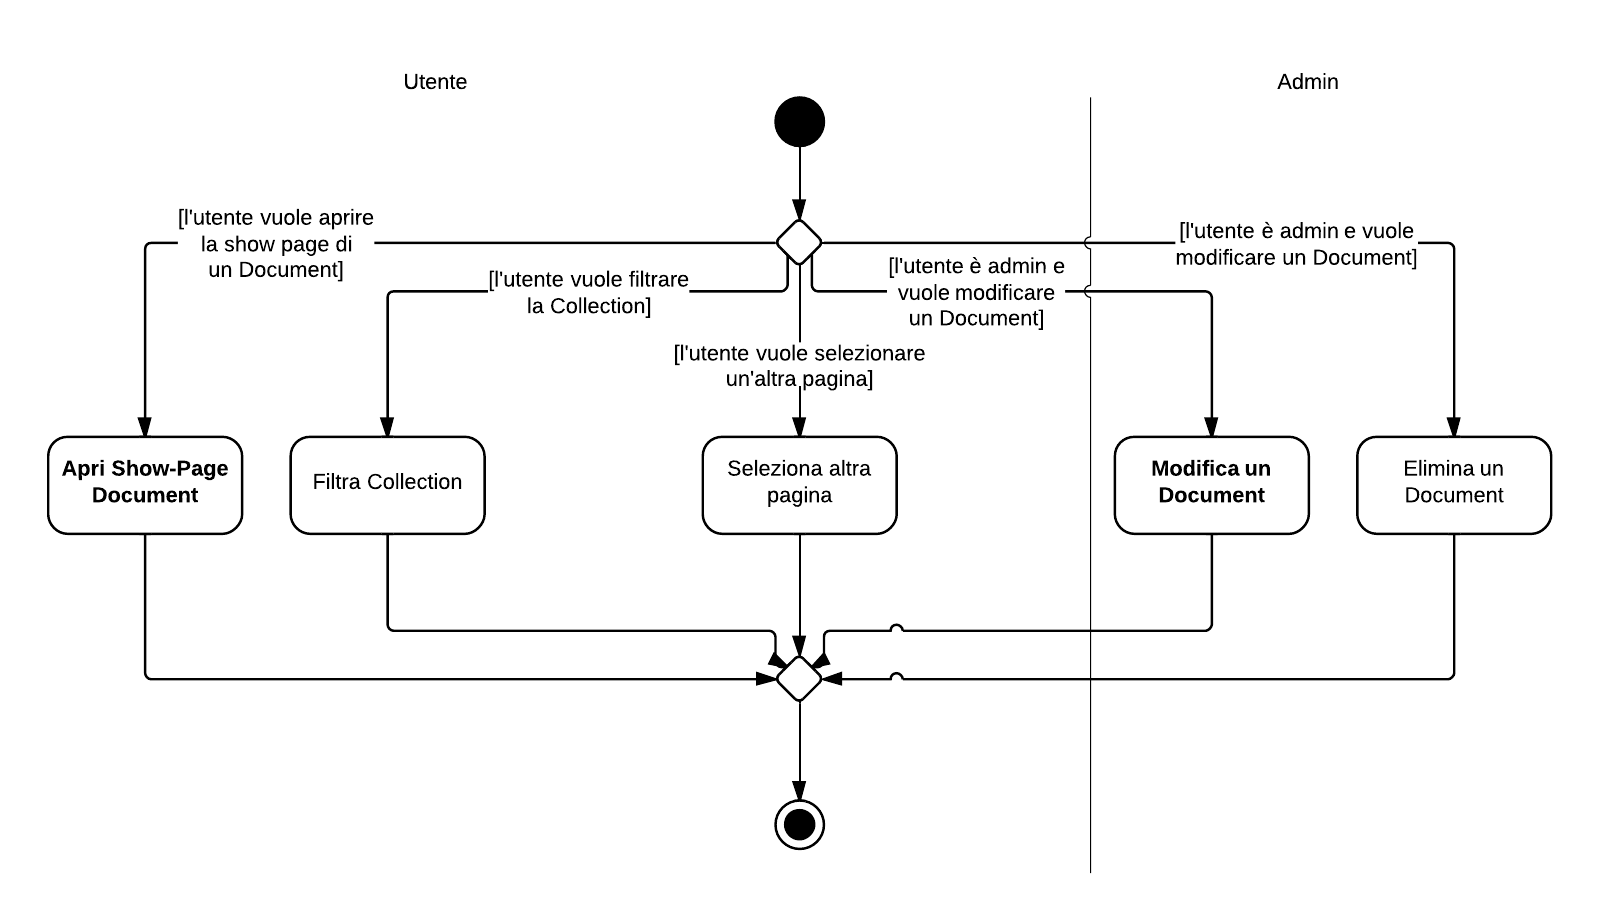
\includegraphics[scale=0.2]{uml/attivita/MaaP - Index-page.png}
\caption{Diagramma di attività - Visualizzazione index-page della Collection selezionata}
\end{figure}

L'utente ha selezionato una \glossario{Collection} dal menu e ora si trova all'interno di una pagina che visualizza una tabella contenente tutti i \glossario{Document} della \glossario{Collection} con alcuni attributi visualizzabili. A questo punto è in grado di fare diverse operazioni:

\begin{itemize}

	\item Può aprire la relativa \glossario{show-page} di un \glossario{Document} selezionando il link che la apre;
	\item Può applicare un filtro ai \glossario{Document} visualizzati in modo da visualizzare un sottoinsieme della tabella;
	\item Se la tabella risulta distribuita su più pagine può accedere alle pagine successive;

\end{itemize}

Se l'utente dispone dei privilegi di admin può inoltre:

\begin{itemize}

	\item Modificare un \glossario{Document} cliccando sul link \textit{edit} visualizzato in ciascuna riga della tabella;
	\item Eliminare un \glossario{Document} cliccando sul link \textit{delete} visualizzato in ciascuna riga della tabella;

\end{itemize}

\subsubsection{Show-page Document}

\begin{figure}[H]
\centering
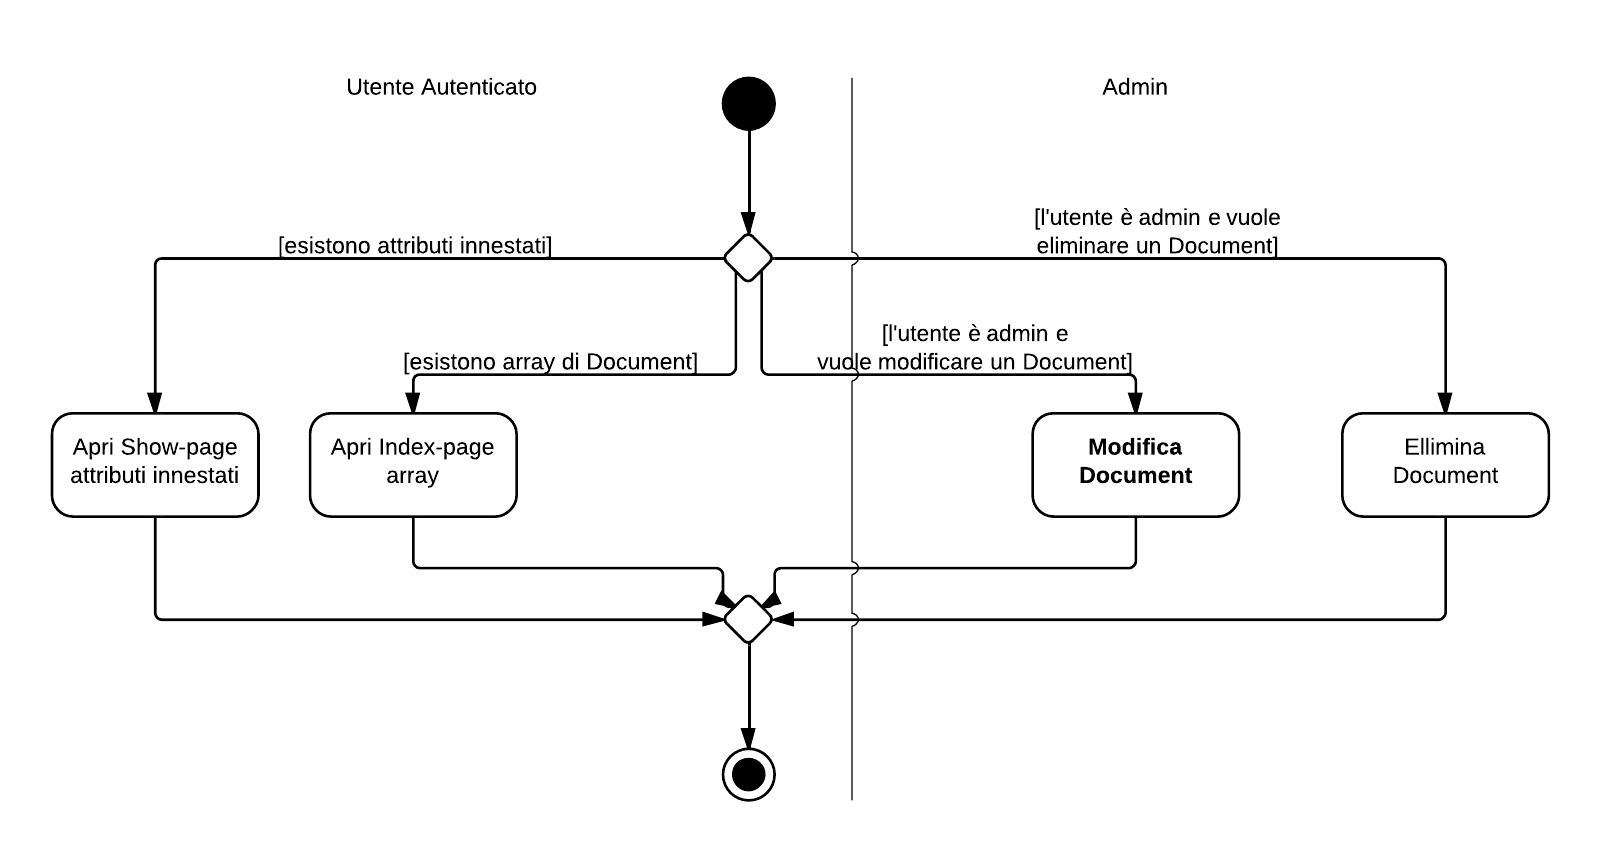
\includegraphics[scale=0.2]{uml/attivita/MaaP - Show-page.png}
\caption{Diagramma di attività - Visualizzazione show-page del Document selezionato}
\end{figure}

L'utente ha selezionato un \glossario{Document} dalla \glossario{index-page} e ora si trova davanti una pagina di visualizzazione dettagliata del \glossario{Document} selezionato. Sostanzialmente questa pagina conterrà una tabella contenente gli attributi visualizzabili del \glossario{Document}. Un utente all'interno di questa pagina può:

\begin{itemize}

	\item Aprire la \glossario{show-page} di un attributo innestato, se ne esiste uno;
	\item Aprire la \glossario{index-page} di un array di \glossario{Document}, se ne esiste uno.

\end{itemize}

Se l'utente possiede i privilegi di admin può inoltre:

\begin{itemize}

	\item Modificare gli attributi del \glossario{Document};
	\item Eliminare il \glossario{Document} corrente.

\end{itemize}

\subsubsection{Apri pagina gestione utenti}

\begin{figure}[H]
\centering
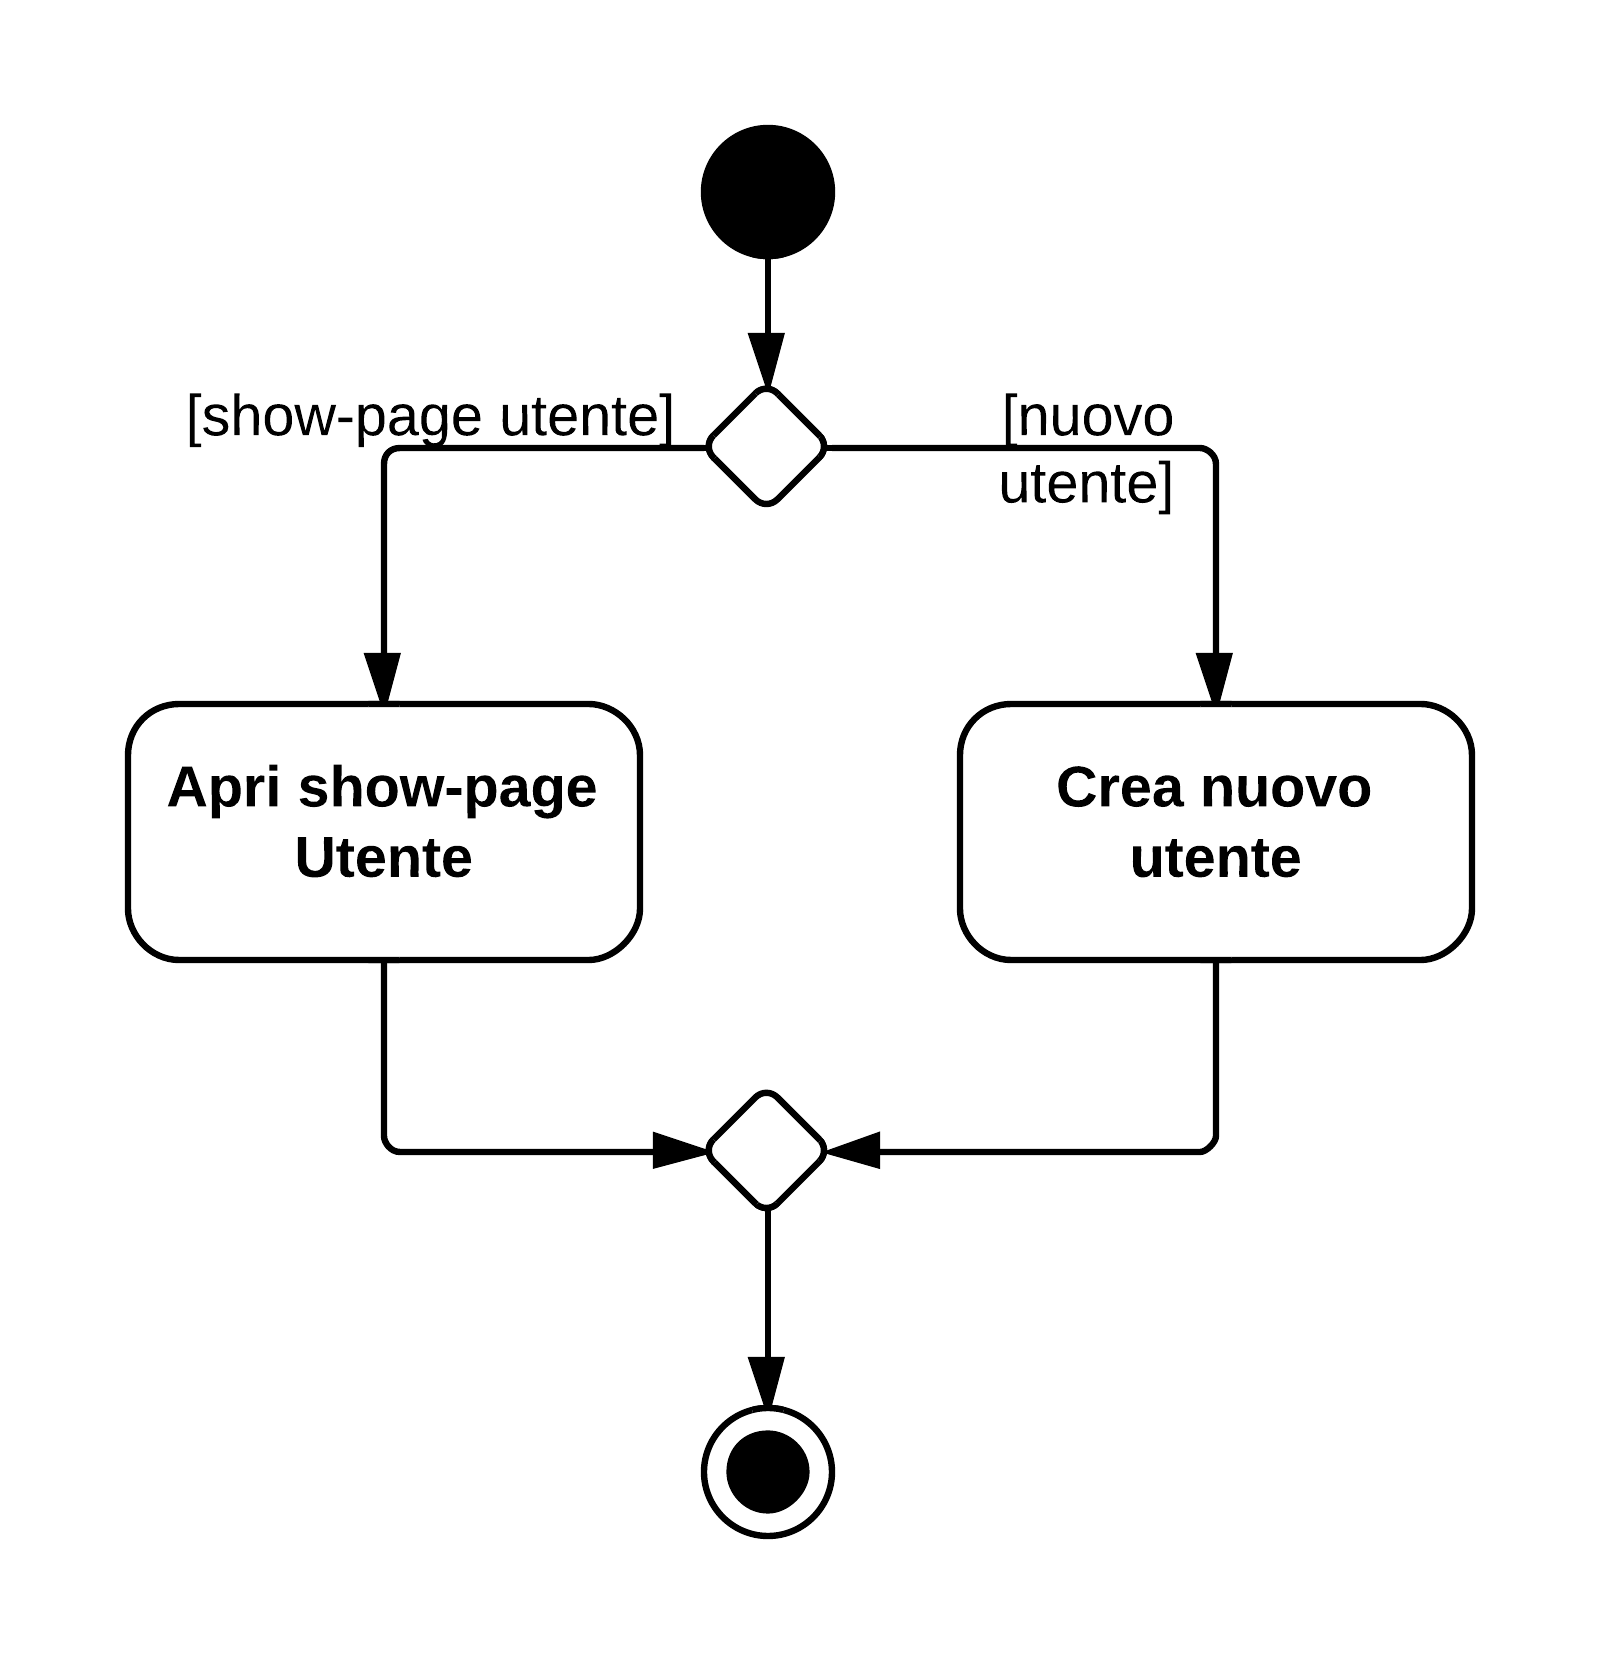
\includegraphics[scale=0.1]{uml/attivita/MaaP - Apri pagina gestione utenti.png}
\caption{Diagramma di attività - Pagina di gestione degli utenti}
\end{figure}

Un admin dell'applicazione può accedere a una pagina in cui poter gestire gli utenti. Essa consiste fondamentalmente in una \glossario{index-page} contenente la lista di tutti gli utenti presenti nel sistema. L'admin può da questa pagina selezionare un utente, e visualizzare quindi la sua relativa \glossario{show-page}, o crearne uno nuovo aprendo la pagina di creazione.

\subsubsection{Apri show-page utente}

\begin{figure}[H]
\centering
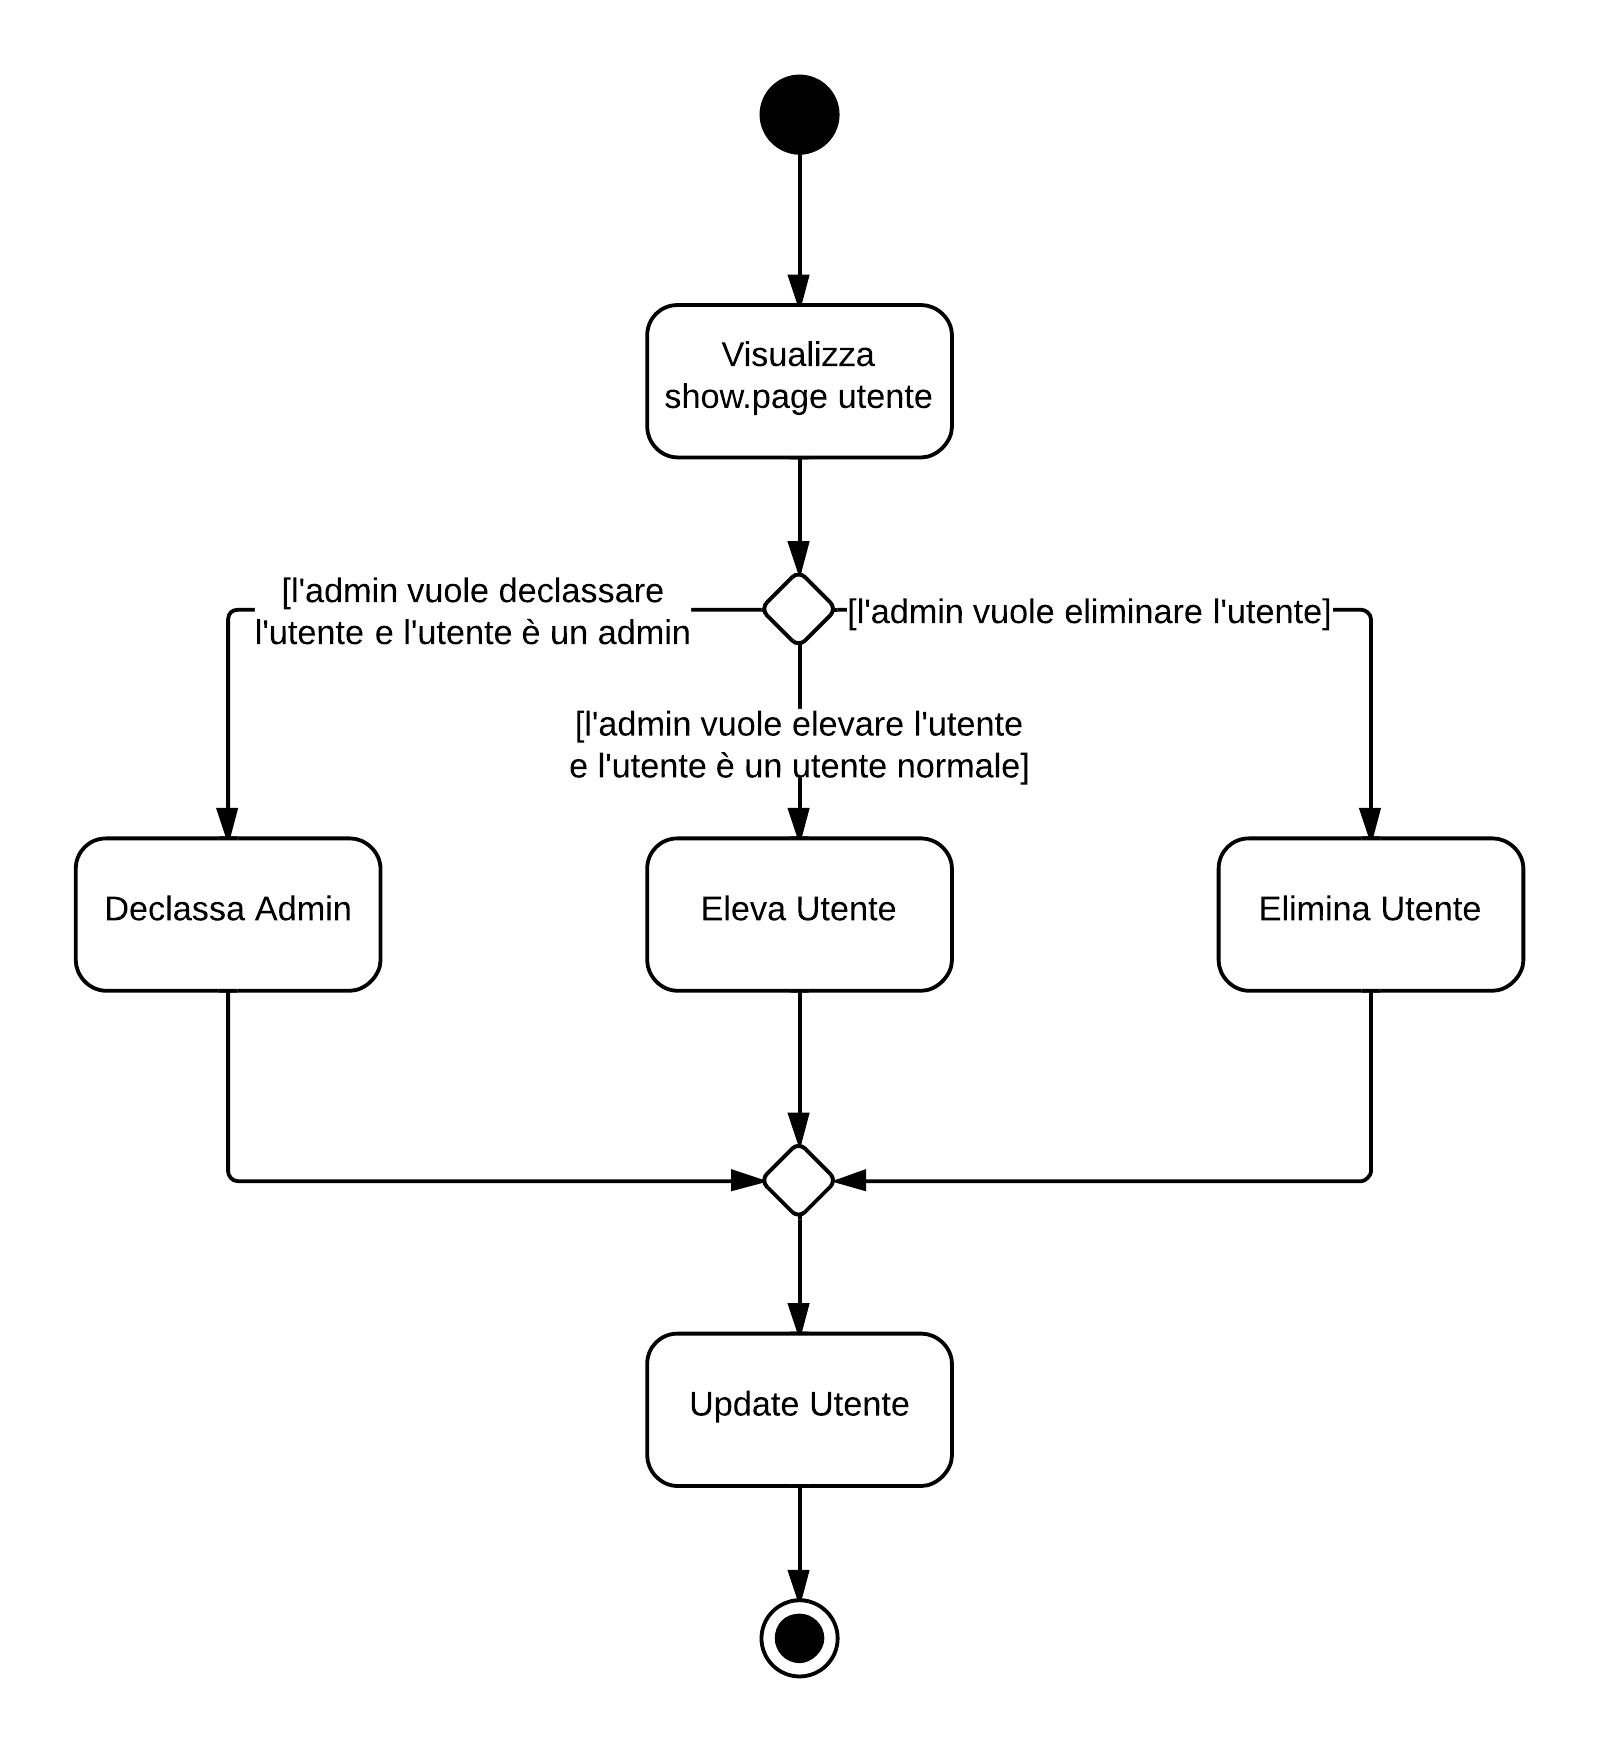
\includegraphics[scale=0.2]{uml/attivita/MaaP - Apri show-page utente.png}
\caption{Diagramma di attività - Pagina di visualizzazione di un utente}
\end{figure}

In questa pagina l'admin visualizza la \glossario{show-page} dell'utente selezionato e può compiere le seguenti operazioni:

\begin{itemize}

	\item Se l'utente selezionato è un admin può declassarlo e portarlo a livello di utente normale. Naturalmente non può declassare se stesso e il \textit{super-admin}, in modo da far sì che in qualsiasi momento sia presente almeno un admin nel sistema;
	\item Se l'utente non è un admin può elevarlo da utente normale a livello di admin;
	\item Eliminare l'utente selezionato dal sistema.

\end{itemize}

Il sistema \glossario{MaaP} si occuperò di apportare tutte le modifiche effettuate dall'admin al \glossario{database} delle credenziali.

\subsubsection{Crea un nuovo utente}

\begin{figure}[H]
\centering
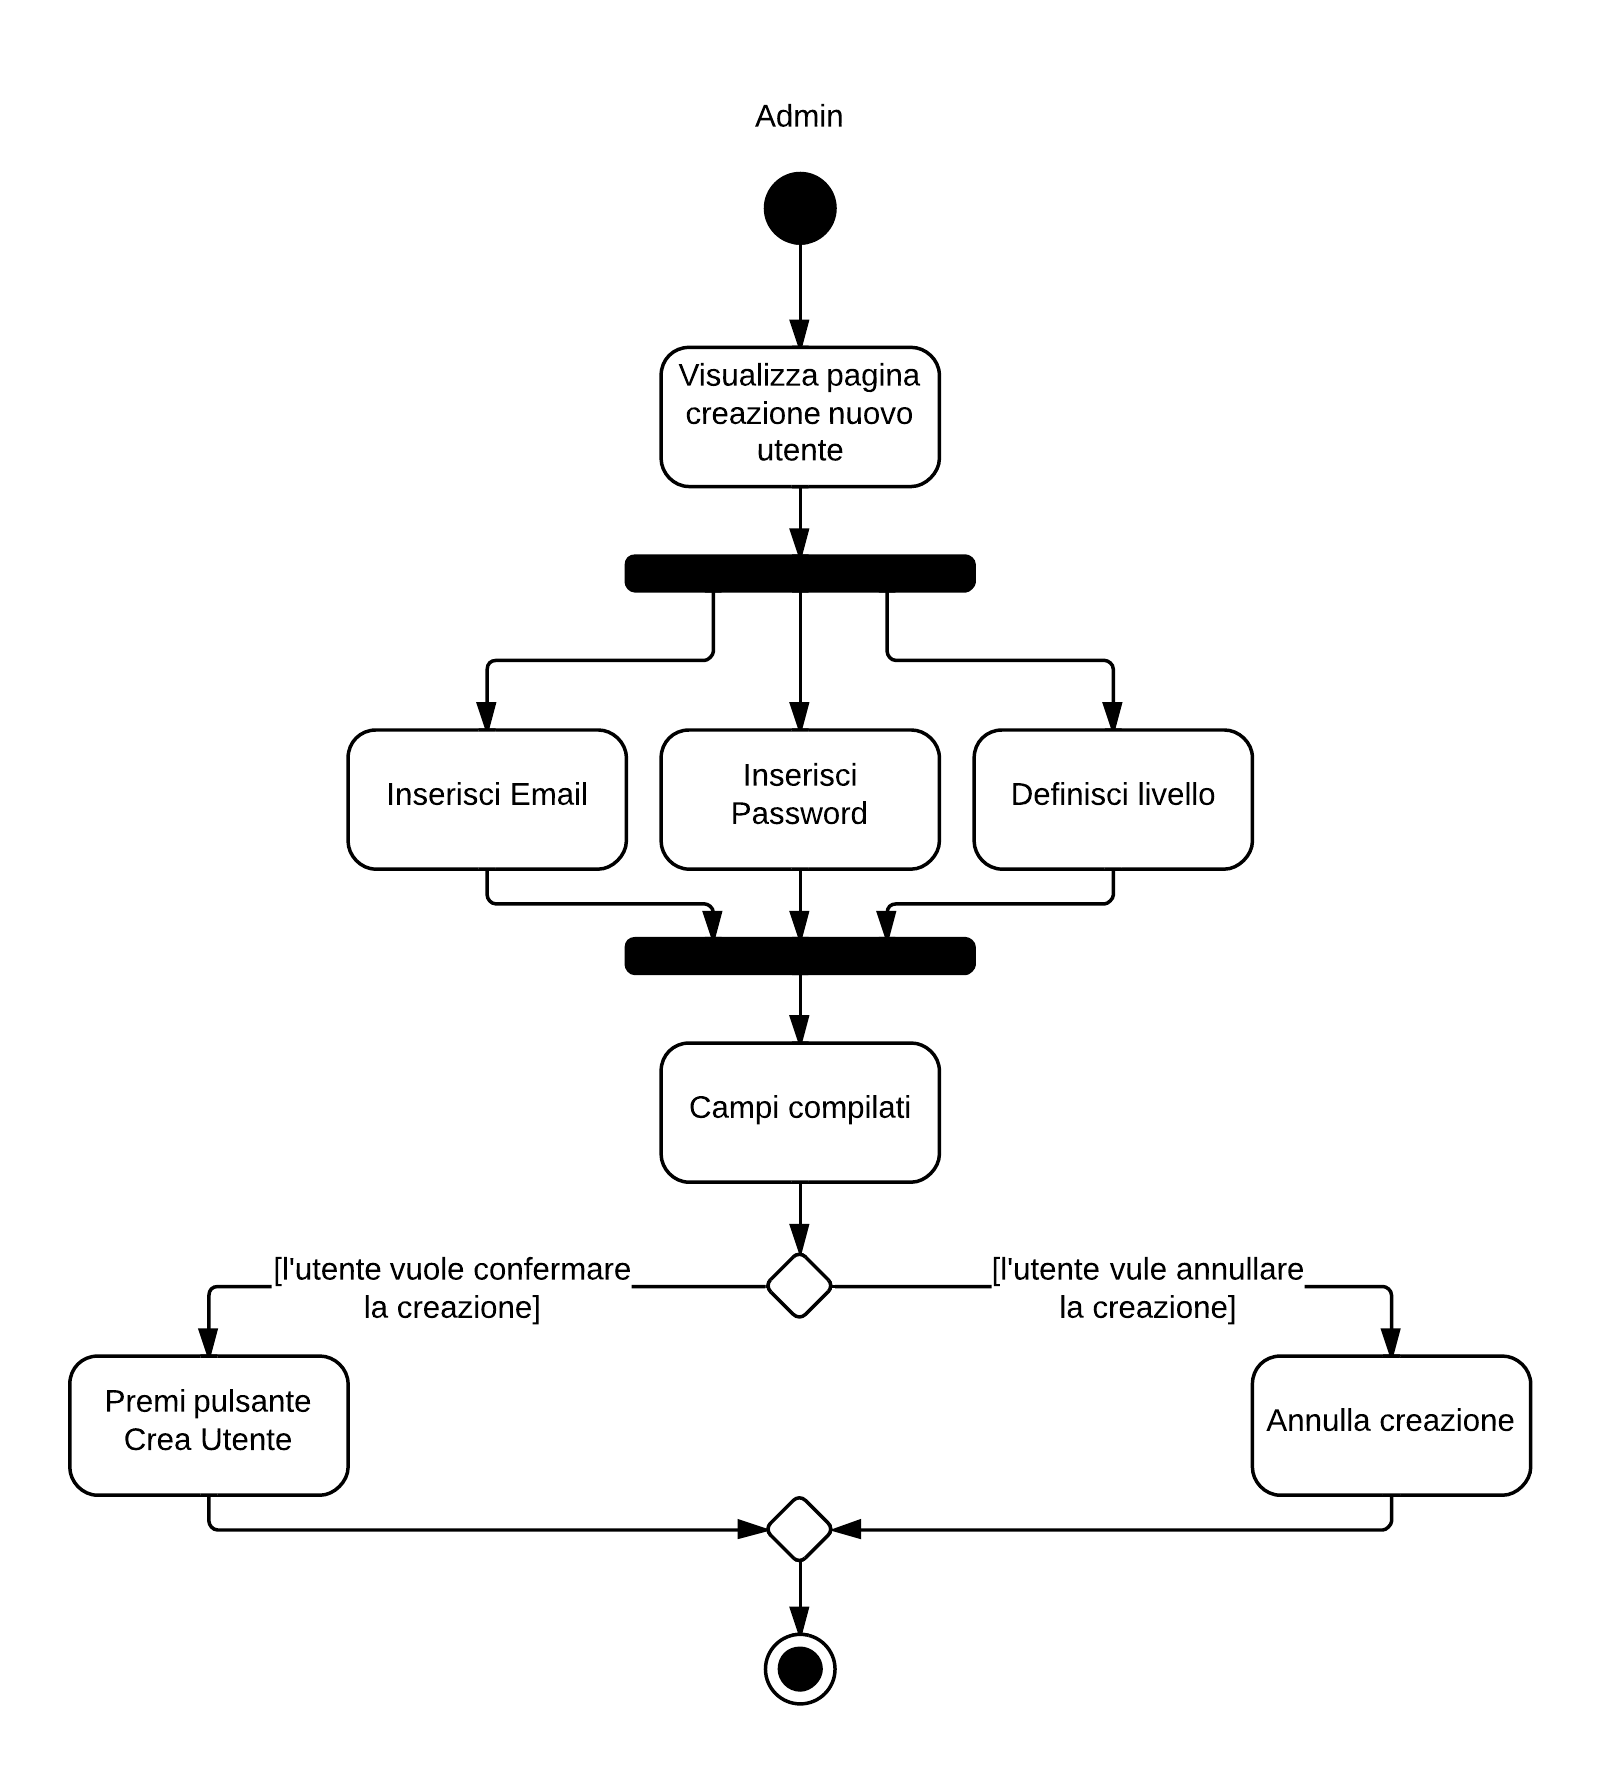
\includegraphics[scale=0.2]{uml/attivita/MaaP - Crea nuovo utente.png}
\caption{Diagramma di attività - Pagina di creazione di un nuovo utente}
\end{figure}

L'admin entra in un'apposita pagina di creazione di un nuovo utente e al suo interno può definire:

\begin{itemize}

	\item L'indirizzo email del nuovo utente;
	\item La password del nuovo utente;
	\item Il livello del nuovo utente, che potrà essere o utente normale o admin;

\end{itemize}

Una volta completate le modifiche l'utente può decidere di confermare o annullare le modifiche, premendo i relativi pulsanti. Il sistema \glossario{MaaP}, nel caso in cui l'utente abbia deciso di confermare le modifiche, si occuperà di inserire nel \glossario{database} delle credenziali il nuovo utente creato.

%\subsection{Servizio MaaS}
%
%Vengono di seguito descritte tutte le iterazioni che un utente può effettuare con il servizio web \glossario{MaaS}.
%
%\subsubsection{attivita principali}
%
%\begin{figure}[H]
%\centering
%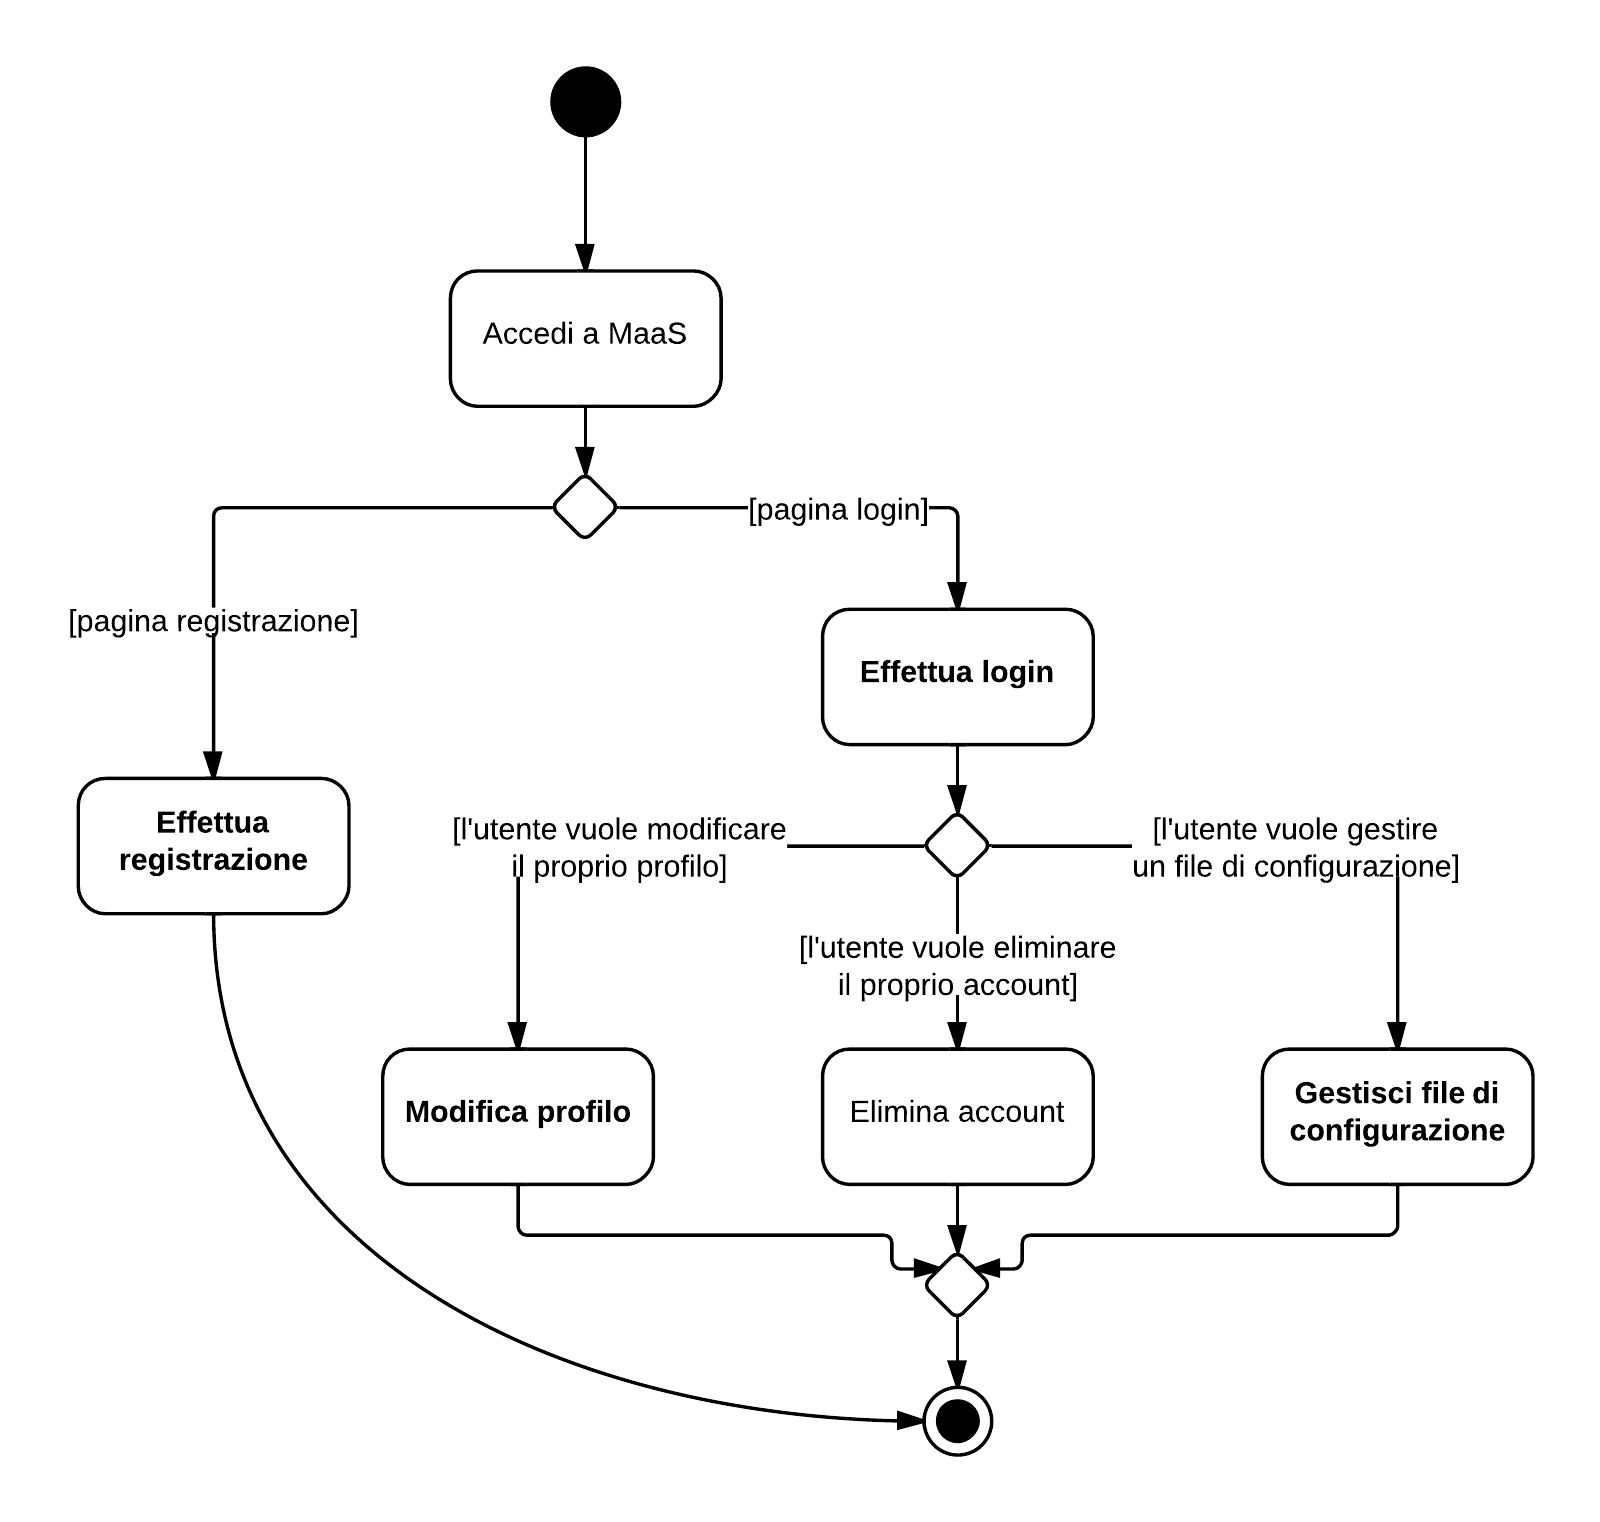
\includegraphics[scale=0.2]{uml/MaaS - Attivita principali.png}
%\caption{Diagramma di attivita - attivita principali di MaaS}
%\end{figure}
%
%L'utente sviluppatore accede tramite il proprio browser al servizio \glossario{MaaS}, il quale gli richiederà l'autenticazione o gli offrirà la possibilità di registrarsi presso di esso. Una volta effettuato l'accesso l'utente si trova di fronte alla propria pagina personale, dalla quale può navigare su altre pagine. Può sostanzialmente effettuare le seguenti operazioni:
%
%\begin{itemize}
%
%	\item Modificare il proprio profilo, cambiando la password di accesso;
%	\item Eliminare il proprio account, eliminando di conseguenza tutti i file di configurazione ad esso associati;
%	\item Gestire i propri file di configurazione della propria applicazione.
%
%\end{itemize}
%
%\subsubsection{Effettua registrazione}
%
%\begin{figure}[H]
%\centering
%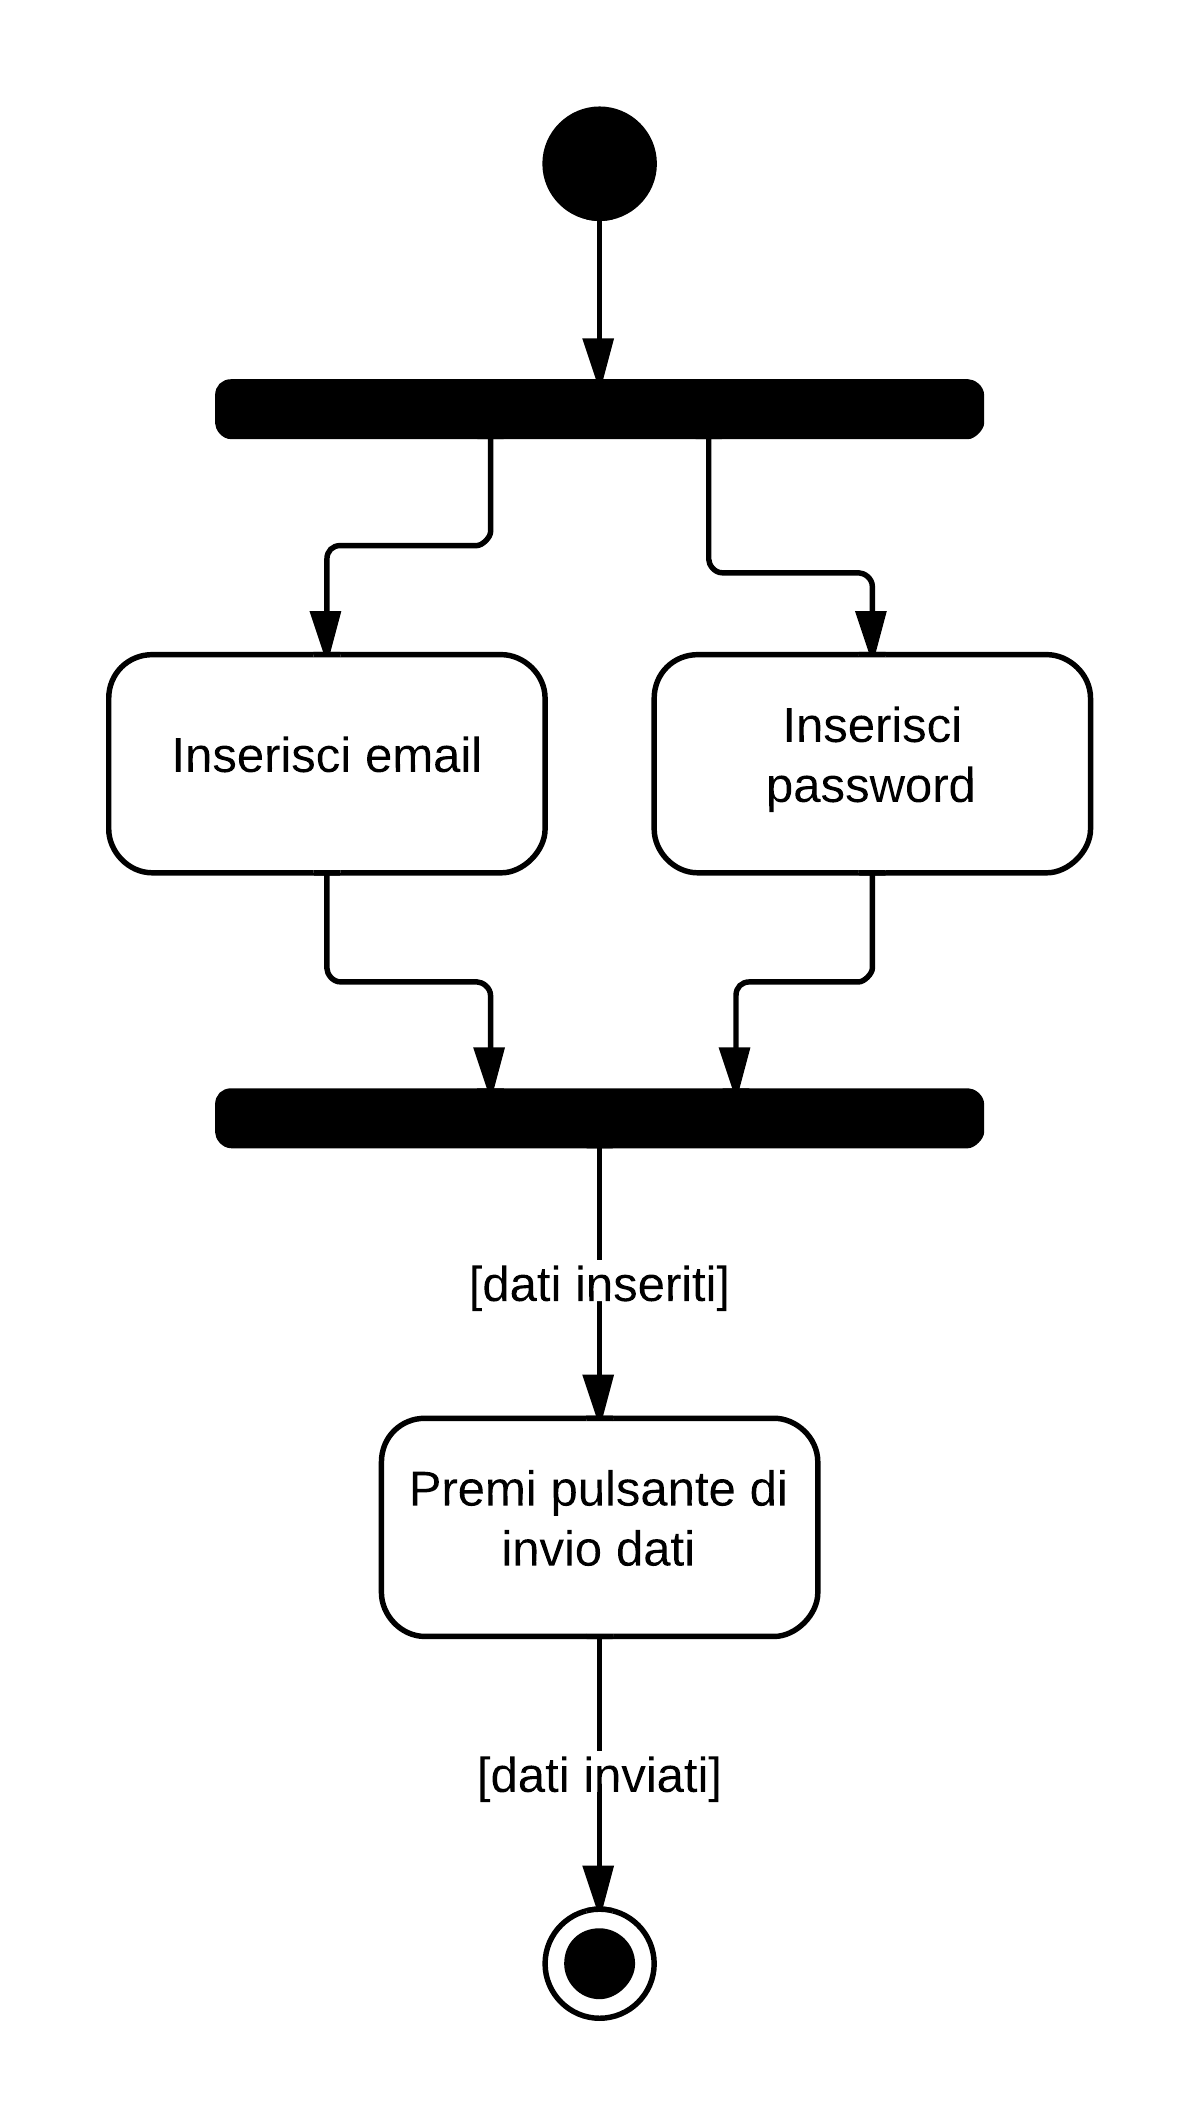
\includegraphics[scale=0.1]{uml/MaaP - Effettua registrazione.png}
%\caption{Diagramma di attivita - Registrazione al servizio MaaS}
%\end{figure}
%
%In maniera pressoché identica da quanto offerto da un'applicazione \glossario{MaaP} l'utente visualizza una pagina di registrazione nella quale deve inserire in appositi campi di testo l'email e la password con le quali vuole registrarsi al servizio. Una volta inseriti i dati premerà il pulsante di richiesta registrazione. Il sistema procederà dunque alla verifica delle credenziali inserite e, se l'indirizzo email non è già presente, procederà alla registrazione del nuovo utente.
%
%\subsubsection{Effettua login}
%
%\begin{figure}[H]
%\centering
%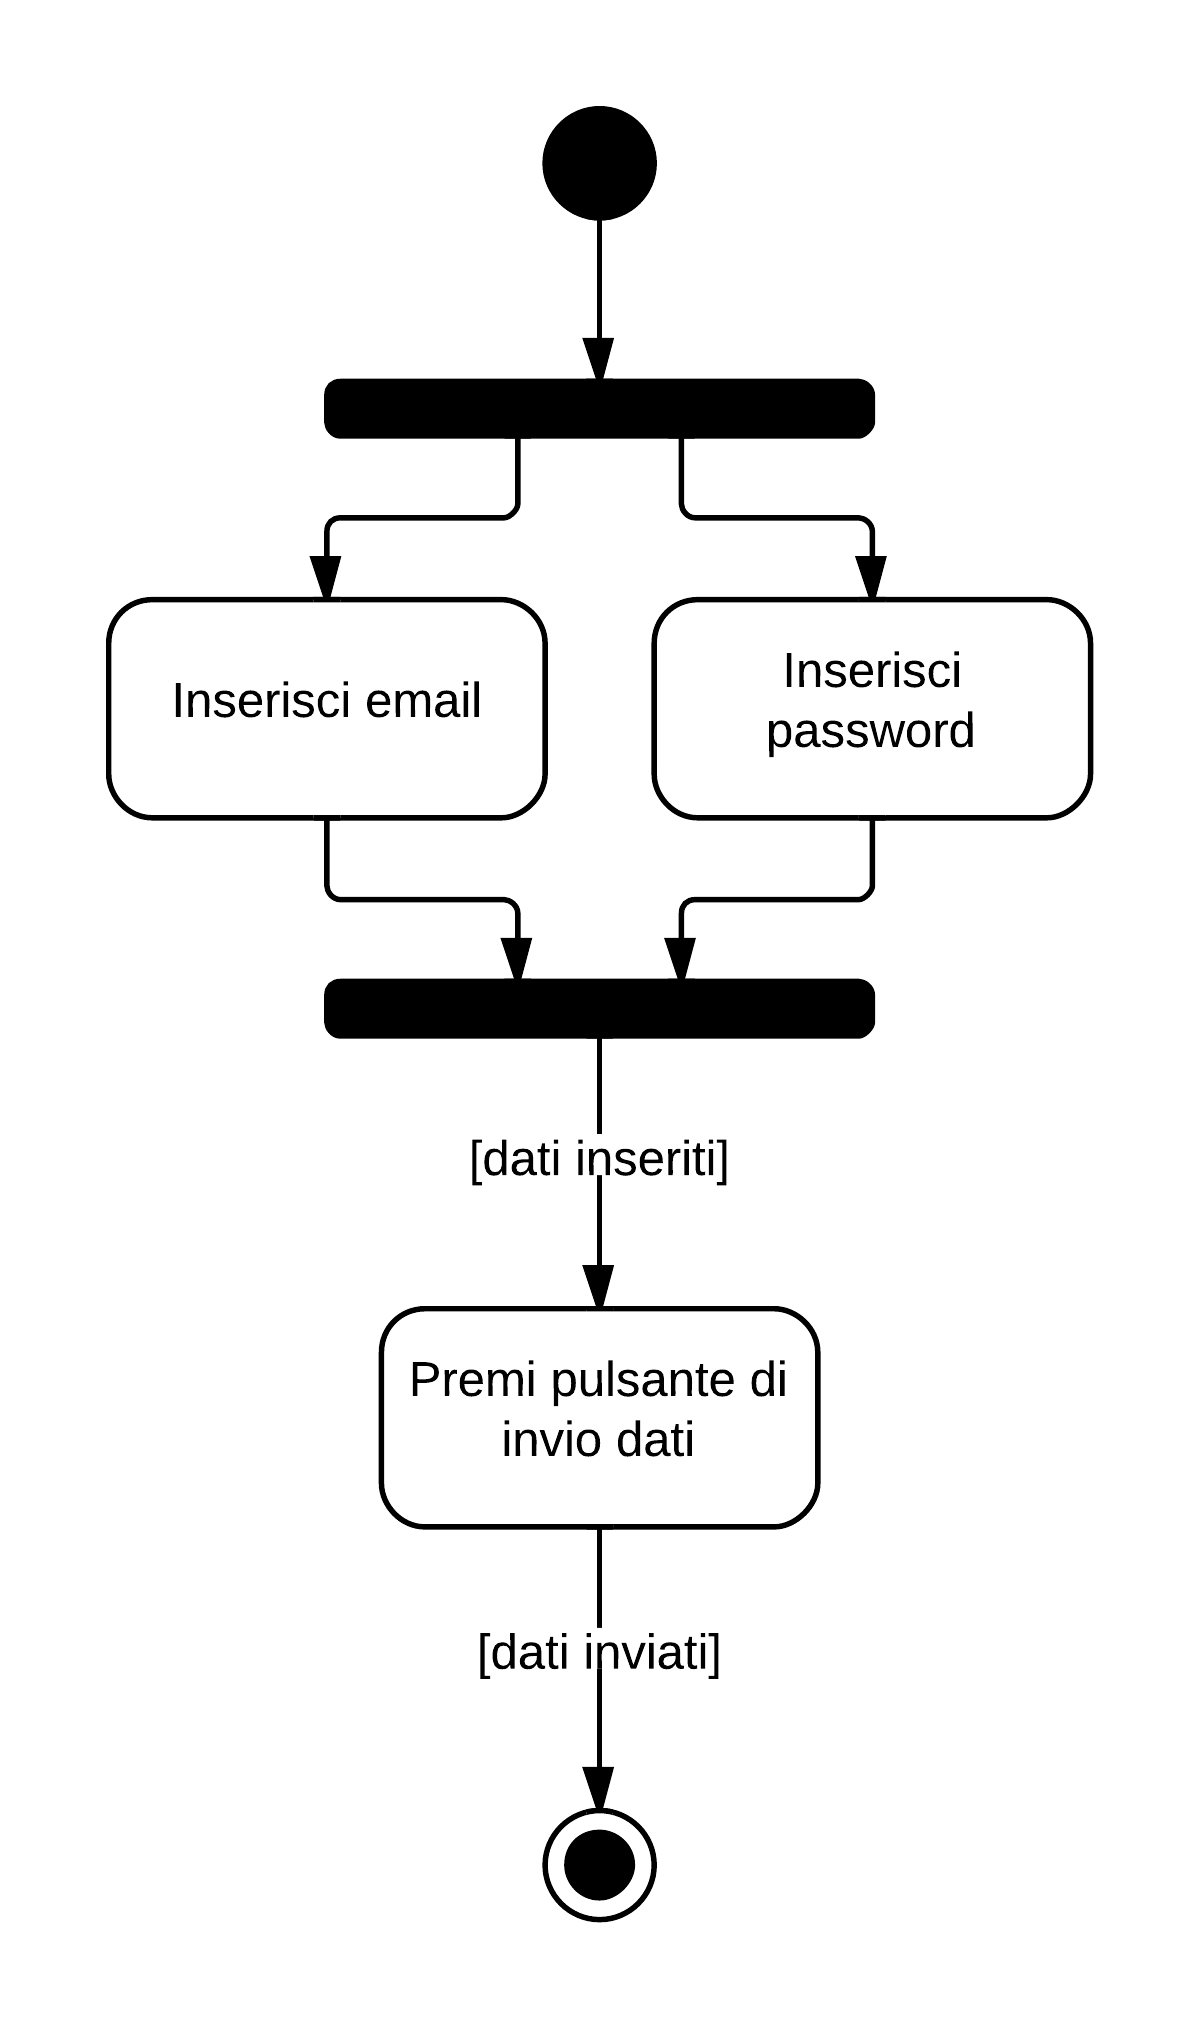
\includegraphics[scale=0.1]{uml/MaaP - Effettua login.png}
%\caption{Diagramma di attivita - Login al servizio MaaS}
%\end{figure}
%
%In maniera pressoché identica da quanto offerto da un'applicazione \glossario{MaaP} l'utente visualizza una pagina di login nella quale deve inserire la propria email e la propria password in appositi campi di testo. Una volta inseriti i dati premerà quindi un pulsante per accedere al servizio \glossario{MaaS}. Il sistema si occuperà di verificare la correttezza delle credenziali e, in caso positivo, effettuerà il login dell'utente.
%
%\subsubsection{Modifica profilo}
%
%\begin{figure}[H]
%\centering
%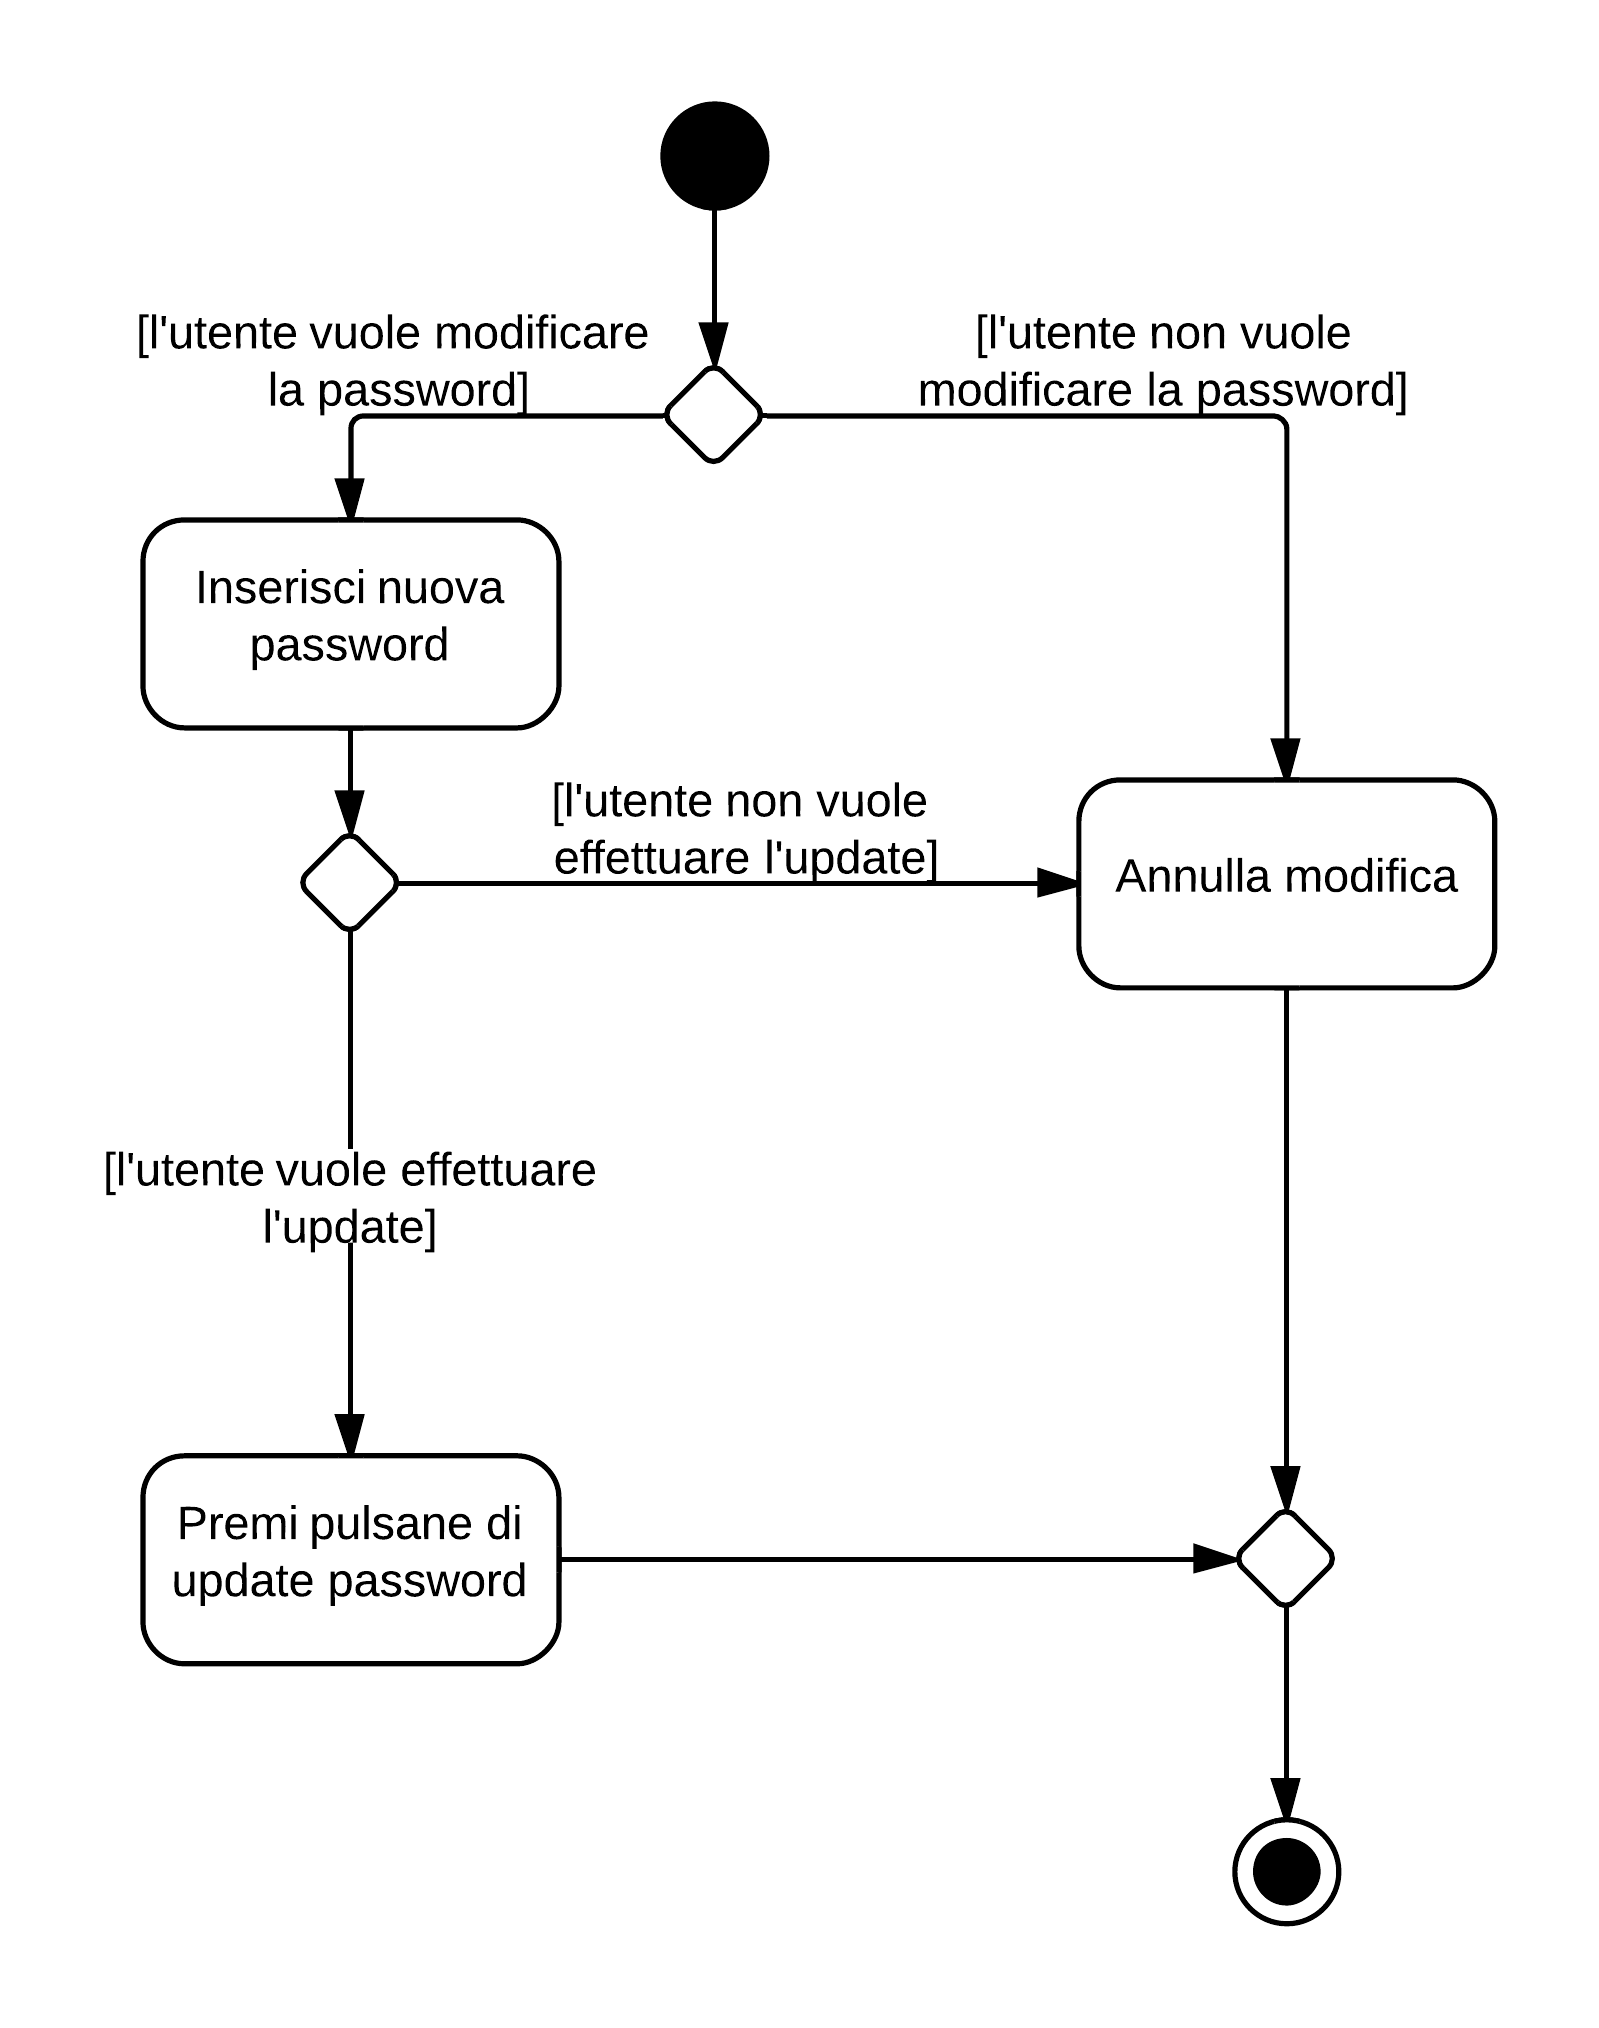
\includegraphics[scale=0.1]{uml/MaaP - Modifica profilo.png}
%\caption{Diagramma di attivita - Modifica profilo dell'utente MaaS}
%\end{figure}
%
%In maniera pressoché identica da quanto offerto da un'applicazione \glossario{MaaP} lo sviluppatore entra all'interno della pagina del proprio profilo, dalla quale può modificare la propria password premendo il relativo pulsante. Se decidesse di non voler modificare può in qualsiasi momento annullare le modifiche premendo l'apposito pulsante. Una volta salvate le modifiche il servizio \glossario{MaaS} si occuperà di effettuare correttamente l'upgrade della password nel \glossario{database} delle credenziali.
%
%\subsubsection{Gestisci file di configurazione}
%
%\begin{figure}[H]
%\centering
%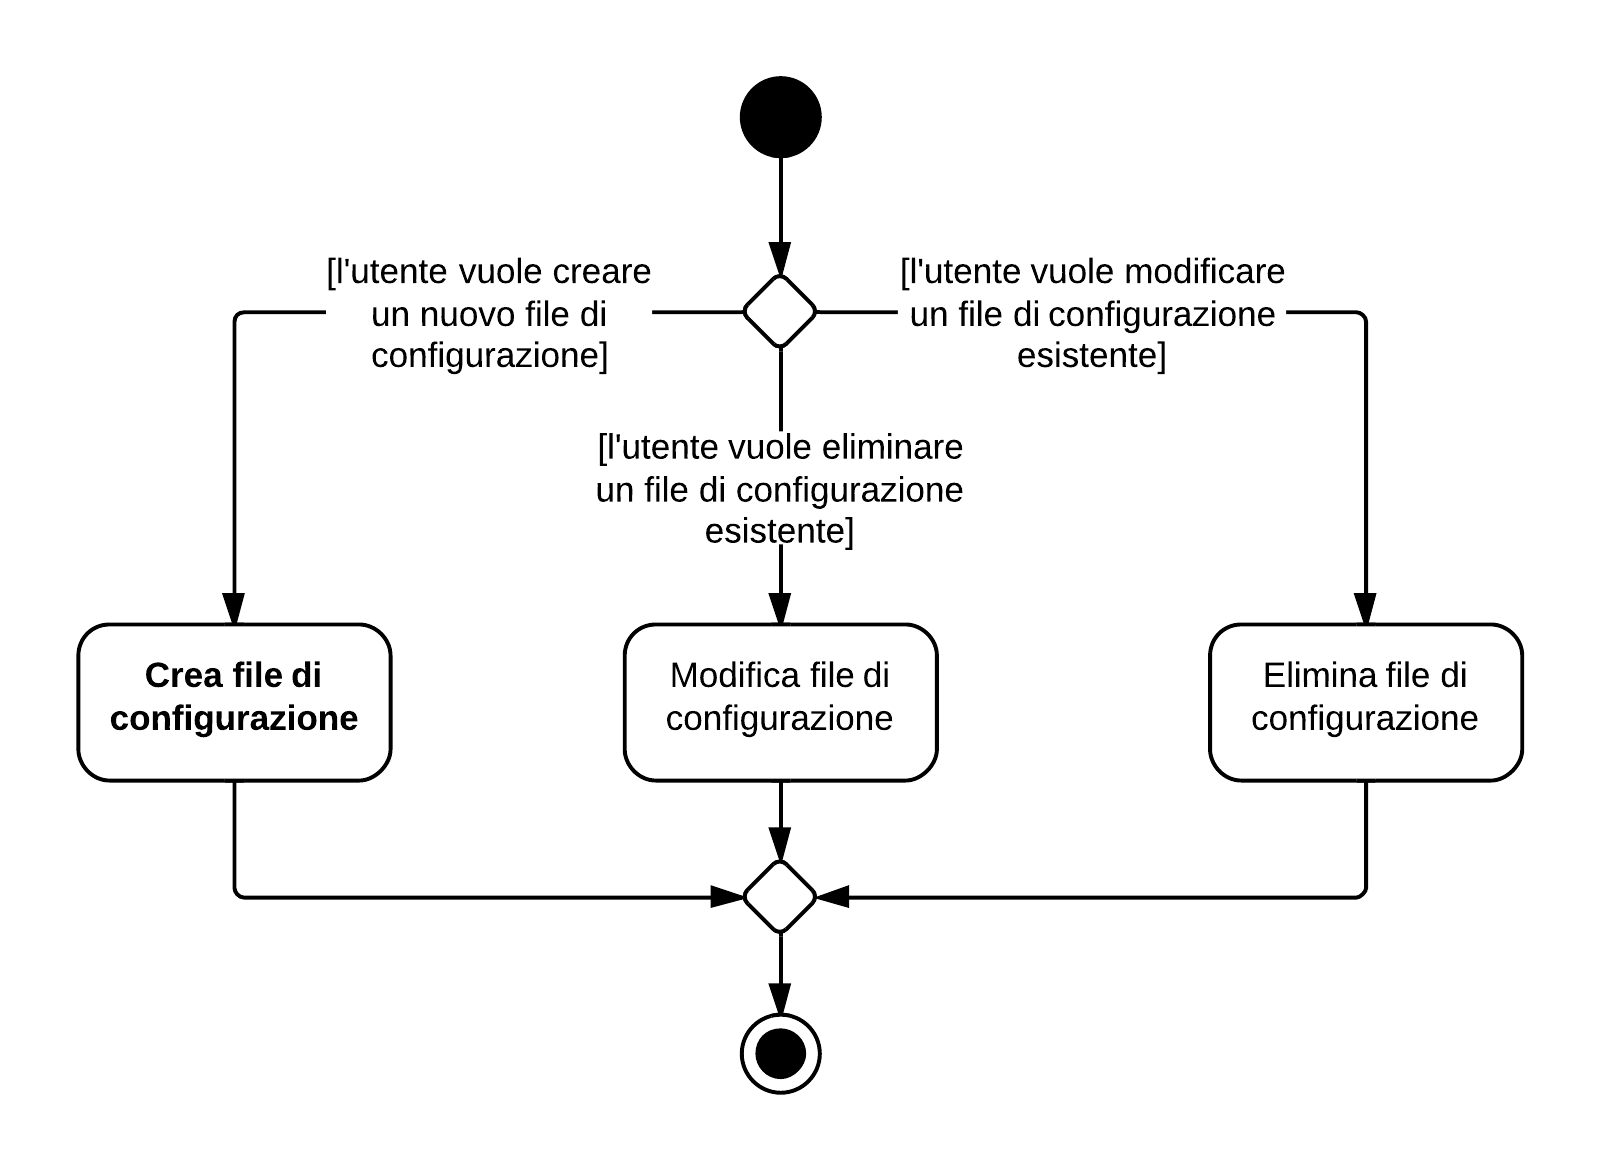
\includegraphics[scale=0.2]{uml/MaaS - Gestisci file di configurazione.png}
%\caption{Diagramma di attivita - Gestione dei file di configurazione}
%\end{figure}
%
%L'utente sviluppatore si trova davanti a una pagina in cui visualizza la lista di tutti i propri file di configurazione presenti. Da questa pagina può decidere di:
%
%\begin{itemize}
%
%	\item Creare un nuovo file di configurazione tramite la procedura descritta in seguito;
%	\item Eliminare un file di configurazione esistente;
%	\item Modificare un file di configurazione esistente in maniera analoga alla creazione.
%
%\end{itemize}
%
%\subsubsection{Crea file di configurazione}
%
%\begin{figure}[H]
%\centering
%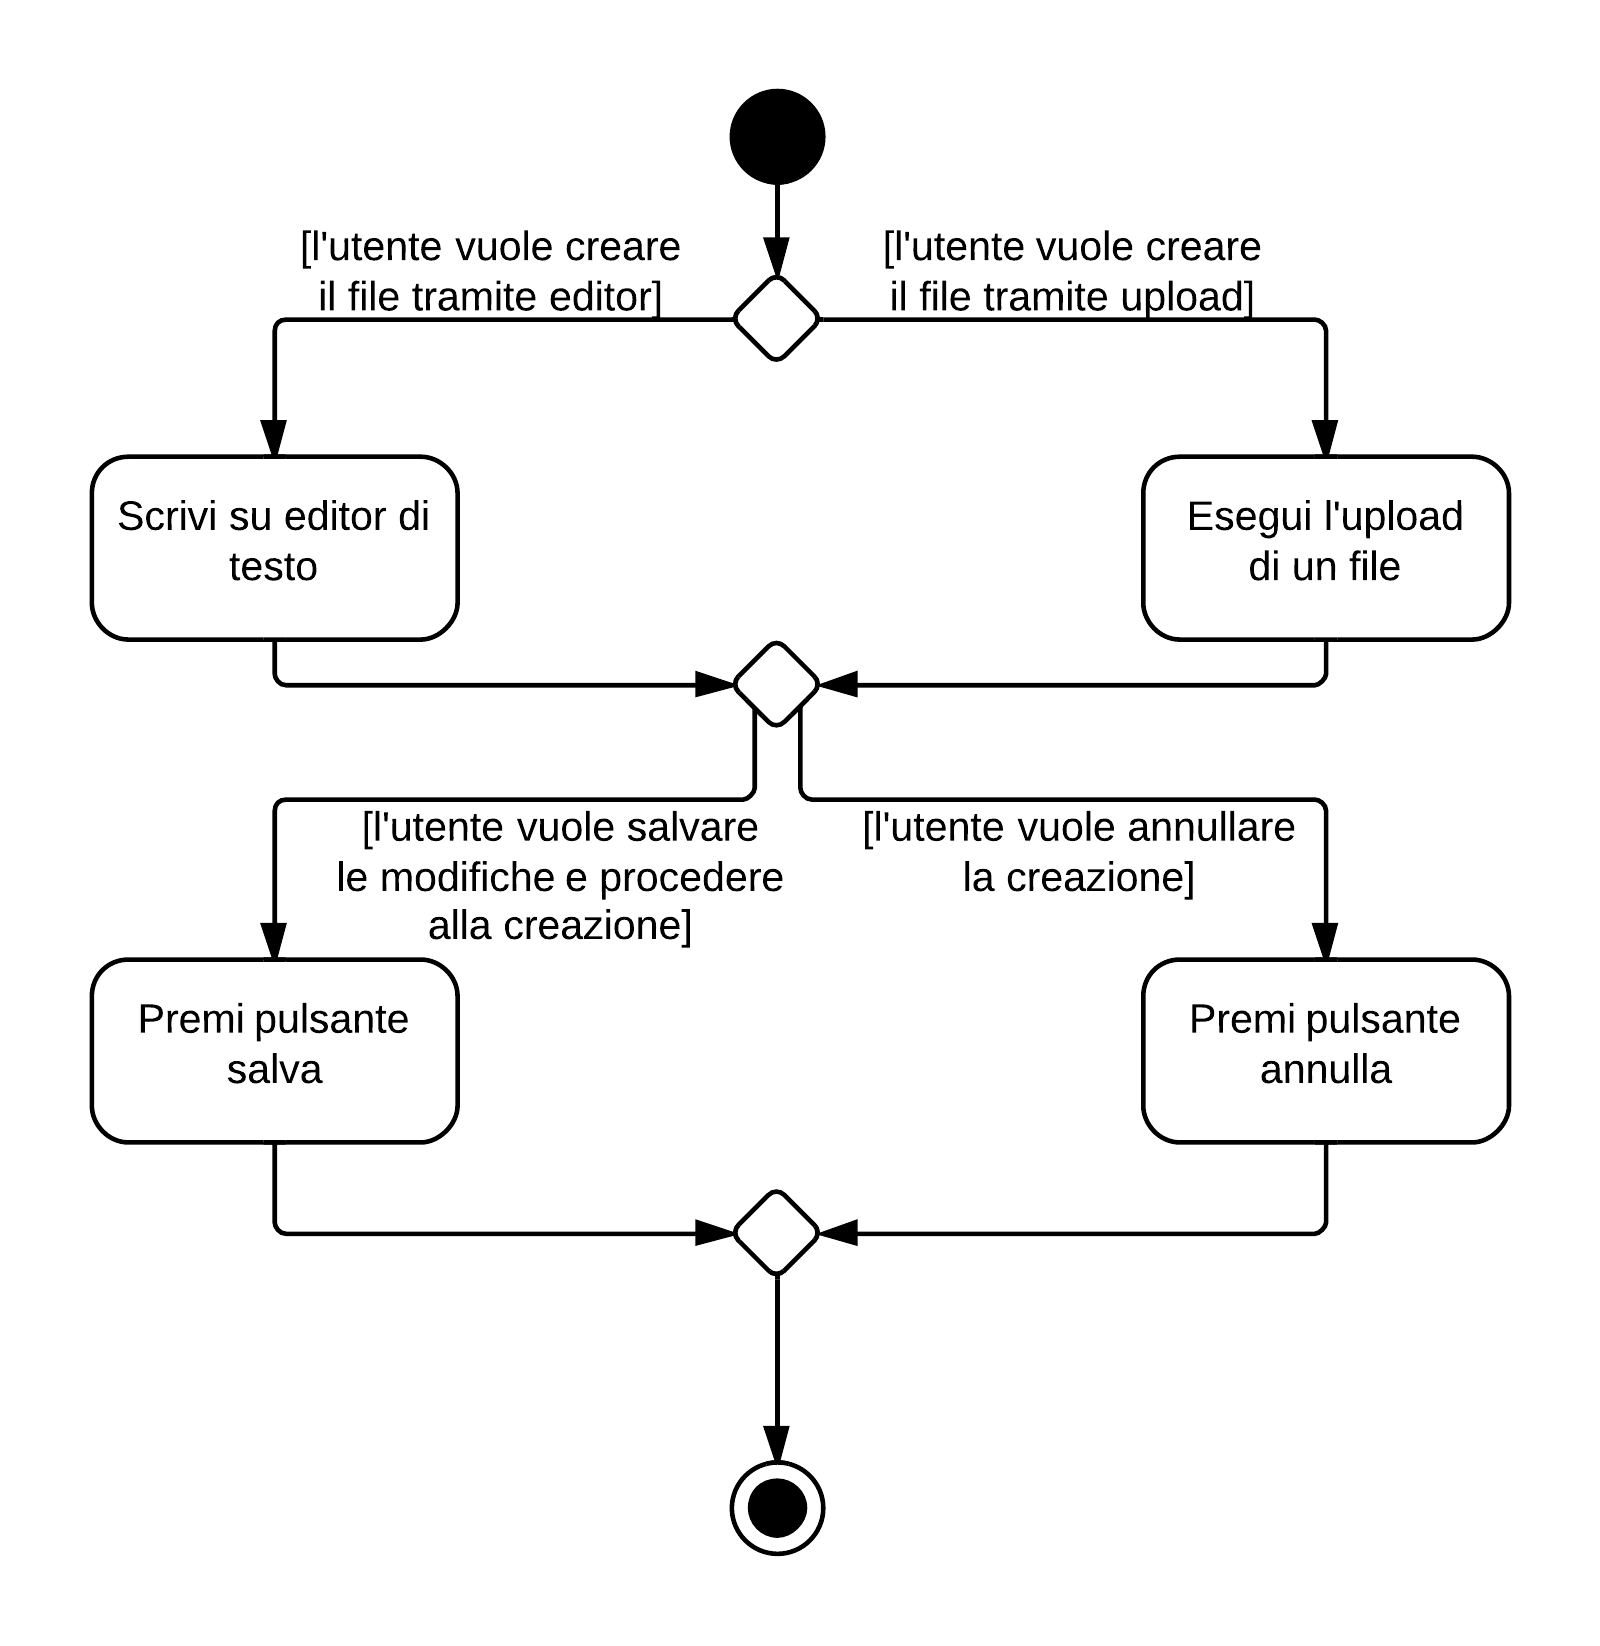
\includegraphics[scale=0.2]{uml/MaaS - Crea file di configurazione.png}
%\caption{Diagramma di attivita - Creazione di un file di configurazione}
%\end{figure}
%
%L'utente sviluppatore si trova davanti a una pagina in cui è presente un editor di testo e un pulsante per effettuare l'upload di un file. Queste sono sostanzialmente le due strade con cui lo sviluppatore può creare un nuovo file di configurazione. Una volta creato o caricato il nuovo file, lo sviluppatore può decidere di procedere al salvataggio oppure annullare la creazione, premendo i relativi pulsanti. Il sistema \glossario{MaaS} nel caso in cui lo sviluppatore decida di procedere alla creazione si occuperà di salvare il file nel sistema.

\subsection{Framework MaaP}

Viene di seguito descritta la procedura con la quale viene creata una nuova applicazione \glossario{MaaP}. Fondamentalmente lo sviluppatore si deve prendere carico di installare tutte le librerie necessarie al corretto funzionamento del \glossario{framework}. Una volta ottenute tutte le \textit{dipendenze} potrà da linea di comando inizializzare un nuovo progetto \glossario{MaaP}. Vengono descritti in seguito i diagrammi di attività per la creazione di una nuova applicazione da parte del sistema.

\subsubsection{Crea nuova applicazione}

\begin{figure}[H]
\centering
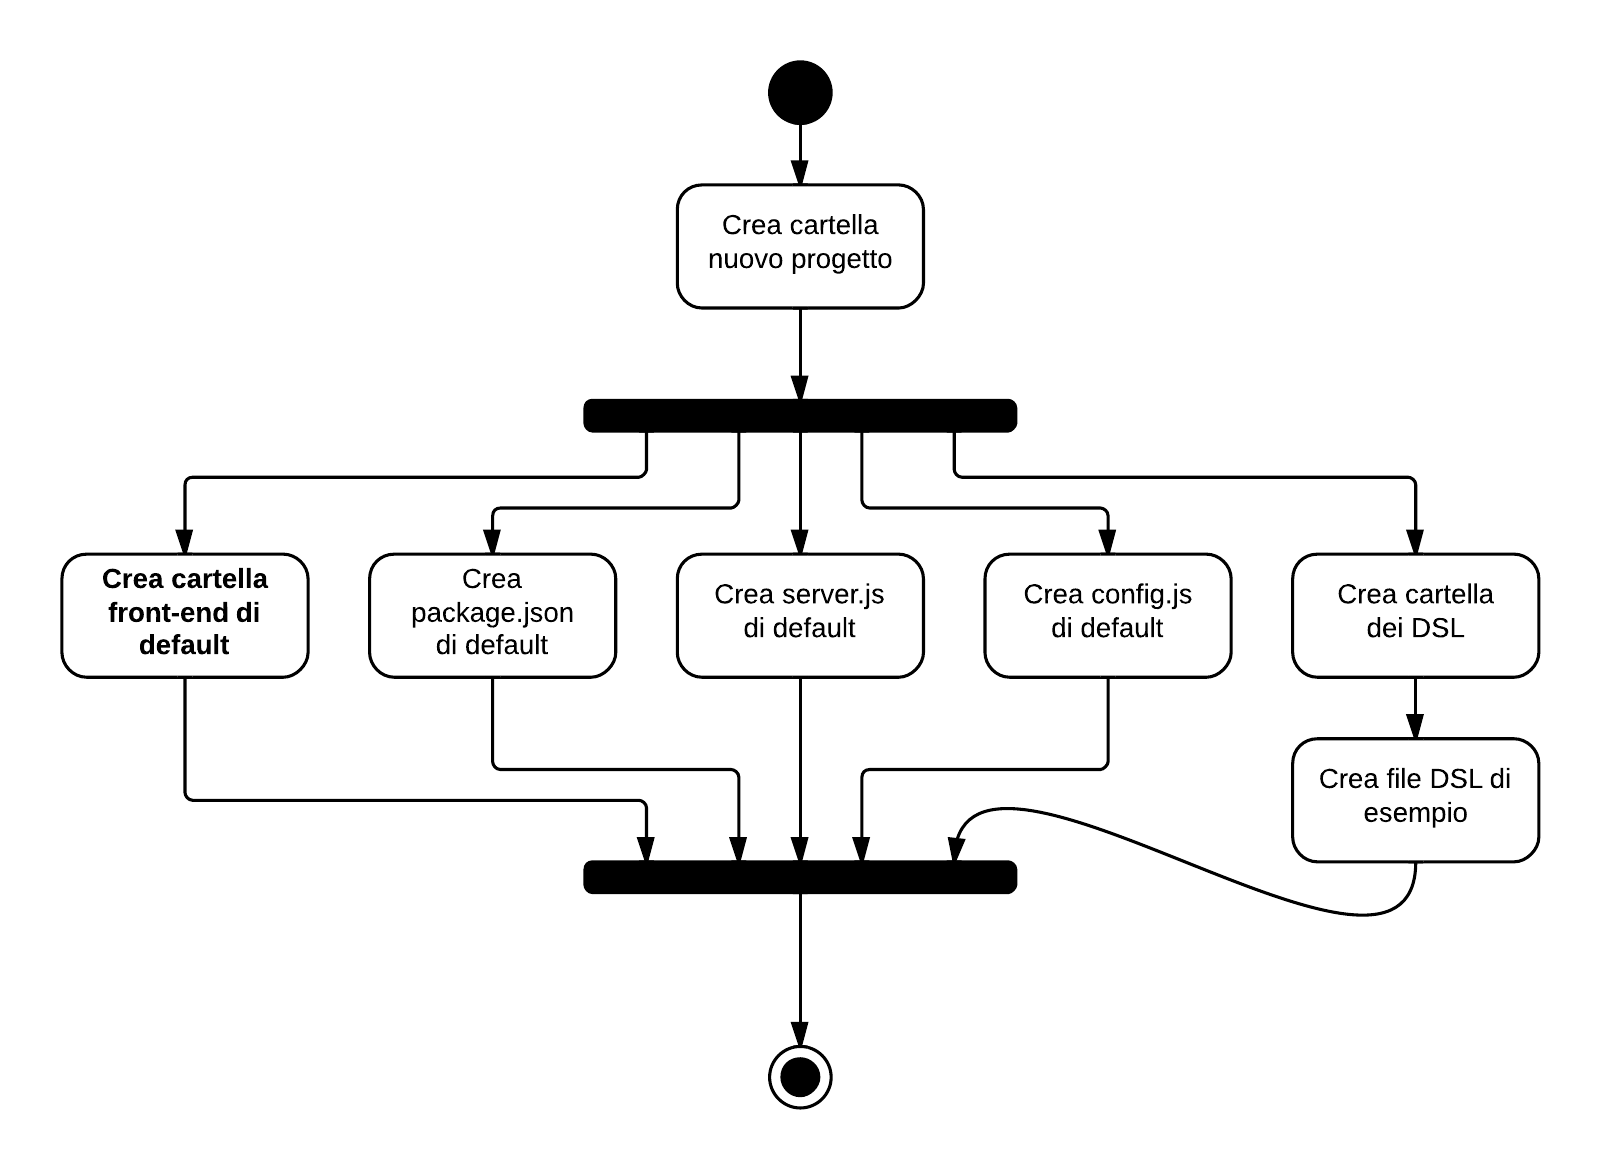
\includegraphics[scale=0.2]{uml/attivita/Framework - Diagramma di installazione.png}
\caption{Diagramma di attività - Creazione scheletro nuova applicazione}
\end{figure}

Il \glossario{framework} \glossario{MaaP} si occupa di creare tutti i file necessari al corretto funzionamento dell'applicazione nella sua versione di \textit{default}. In particolare si occupa di:

\begin{itemize}

	\item Creare una cartella dove andranno tutti i file relativi al \glossario{front-end};
	\item Creare il file \texttt{package.json} di default, nel quale verrà descritta l'applicazione specificando, ad esempio, il nome, le dipendenze, la versione;
	\item Il file \texttt{server.js} di default, il quale fornisce uno script da eseguire per avviare il server;
	\item Il file \texttt{config.js} di default nel quale viene configurata l'applicazione impostando ad esempio i database;
	\item Una cartella contenente tutti i file \glossario{DSL} che lo sviluppatore andrà a configurare. Di default questa cartella conterrà inizialmente un file \glossario{DSL} di esempio.

\end{itemize}

\subsubsection{Creazione cartella front-end di default}

\begin{figure}[H]
\centering
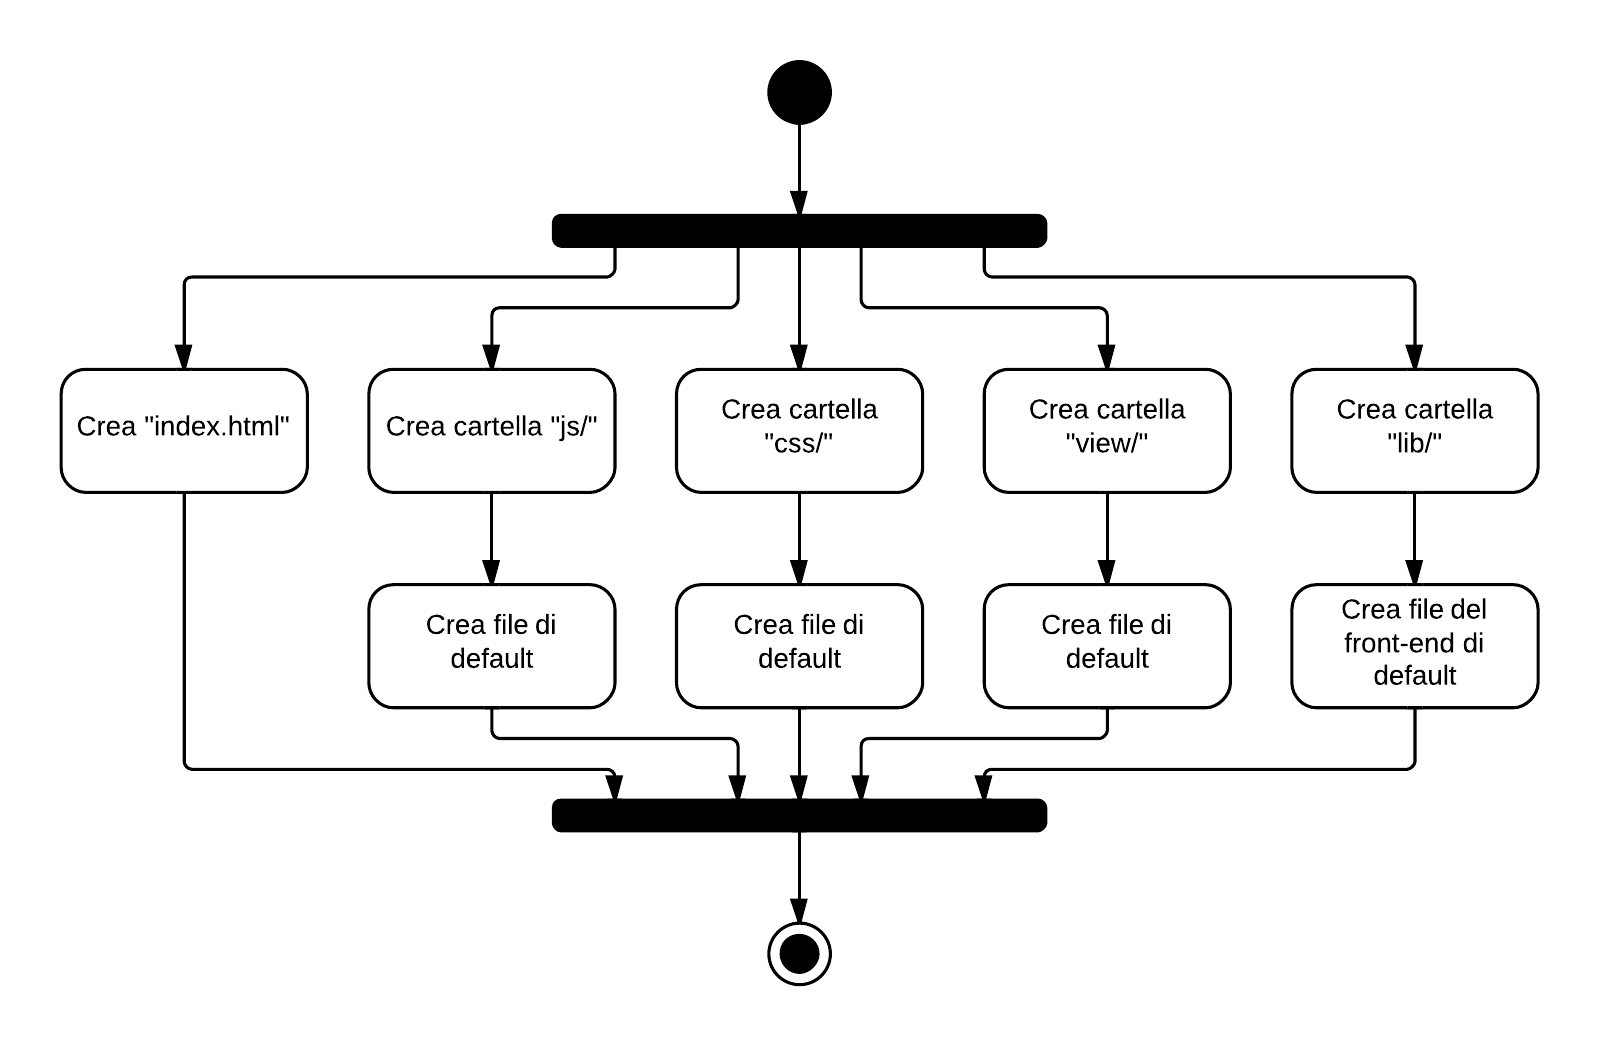
\includegraphics[scale=0.2]{uml/attivita/Framework - Crea cartella front-end di default.png}
\caption{Diagramma di attività - Creazione scheletro nuova applicazione}
\end{figure}

All'interno di questa cartella sono presenti tutti i file di \textit{default} per il corretto funzionamento del front-end. Oltre alla pagina \texttt{index.html} che fungerà da \emph{home} dell'applicazione verrà creato:

\begin{itemize}

	\item La cartella \texttt{js/} all'interno della quale saranno presenti tutti gli script \glossario{javascript} necessari al corretto funzionamento dell'applicazione;
	\item La cartella \texttt{css/} la quale conterrà tutti i fogli di stile per la \textit{presentazione} dell'applicazione;
	\item La cartella \texttt{view/} nella quale saranno presenti i file \textit{html} che fungeranno da \textit{template};
	\item La cartella \texttt{lib/} in cui saranno presenti le librerie \glossario{javascript} già predisposte per il \glossario{front-end}.

\end{itemize}

All'interno di ciascuna cartella saranno presenti inoltre i relativi file di \textit{default}.